\hypertarget{idiopathic-pulmonary-fibrosis-job-exposures-study-ipfjes-is-occupational-asbestos-exposure-an-under-recognised-cause-of-ipf}{%
\section{Idiopathic pulmonary fibrosis job exposures study (IPFJES): Is
occupational asbestos exposure an under-recognised cause of
IPF?}\label{idiopathic-pulmonary-fibrosis-job-exposures-study-ipfjes-is-occupational-asbestos-exposure-an-under-recognised-cause-of-ipf}}

\hypertarget{introduction}{%
\subsection{Introduction}\label{introduction}}

Occult occupational asbestos exposure as a cause for otherwise
`idiopathic' pulmonary fibrosis has been an open question for at least
30 years. It arises because of the clinical and radiological
similarities of asbestosis and IPF; a usual interstitial pneumonia is
observed in both, and patients can present in the same way (chapter 1).
Patients having significant asbestos exposure, that would warrant a
diagnosis of asbestosis, may go undetected because they do not recall
exposure or because where they do recall exposure it is difficult to
assess if it has been sufficient to have caused disease (chapter 4). A
recent meta-analysis of IPF case control studies reporting on
occupational exposures found significant associations between metal,
wood, and stone dust, and IPF (chapter 2). However, the extent of
confounding among groups of workers likely to have significant asbestos
co-exposure, for example metal sheet workers and carpenters, is unknown.
The majority of these studies are limited by their reliance on
self-reported binary exposure which risks recall bias and does not
permit investigation of dose-response relationships which would be
helpful for establishing causality. Studies to date have also not looked
at the possibility of gene-environment interaction; genetic risk factors
such as rs5270590 are now well established and interaction with inhaled
exposures is suspected but has not yet been proven in humans (chapter
5). The question of asbestos exposure in IPF is a live one globally
because countries such as Brazil, Russia, India, and China continue to
consume large quantities of asbestos and, closer to home, asbestos
related and IPF mortality rates continue to rise. While asbestos related
mortality in the UK is driven primarily by pleural mesothelioma and is
expected to peak in the next couple of years as a result of effective
asbestos exposure control legislation, the sustained rise in IPF
mortality rates is unexplained (chapter 3).

\hypertarget{overview}{%
\subsection{Overview}\label{overview}}

IPFJES is a multi-centre, hospital-outpatient, incident case-control
study conceived to address the question of asbestos exposure having a
causal role in IPF. Participants were recruited from a network of 21
hospitals across England, Scotland, and Wales. `Cases' were men who
presented with a new MDT-confirmed diagnosis of IPF consistent with
standard criteria.{[}@Raghu2011{]} Controls were men who attended
randomly selected outpatient clinics in the same time period. Over 460
cases and 460 controls, frequency-matched on age, were recruited to
achieve a predefined recruitment target of 920 participants.
Participants were interviewed by telephone using a bespoke study web
application (ipfjes-interview, full source code available, see Appendix
4). Lifetime occupational history, smoking history, drug history, family
history, and modified Medical Research Council (mMRC) dyspnoea score
were recorded. Each occupation was coded on the basis of the Office for
National Statistics (ONS) standardised occupational classification 1990
(SOC90) at the time of the interview. For participants who recalled
carrying out tasks with asbestos a detailed assessment of each work task
was recorded. SOC90 coded jobs were used to assign asbestos exposure
risk to participants using occupational proportional mortality rates for
malignant pleural mesothelioma. A fibre-ml.year estimate was calculated
for participants recalling asbestos exposure. All participants provided
an EDTA venous blood sample from which DNA was extracted and genotyped
according to known IPF susceptibility SNP rs35705950 using Q-PCR and a
Taqman assay. Unconditional logistic regression was used to analyse
`any' vs `no' asbestos exposure and categories of cumulative exposure
adjusting for age and smoking status. In a secondary analysis I used
unconditional logistic regression to investigate metal, wood, and stone
dust exposure (self-reported occupational exposure), and rs35705950
genotype-exposure interactions.

\hypertarget{method}{%
\subsection{Method}\label{method}}

\hypertarget{funding-approvals-and-registration}{%
\subsubsection{Funding, approvals, and
registration}\label{funding-approvals-and-registration}}

I obtained funding from the Wellcome Trust (201291/Z/16/Z) and NHS
ethical approval (IRAS project ID 203355, REC reference 17/EM/0021). I
also obtained NIHR portfolio status (CPMS ID 203355) and registered the
study on clinicaltrials.gov (NCT03211507). See Appendix 1 for study
protocol, full study documentation is available online at
www.ipfjes.org.

\hypertarget{selection}{%
\subsubsection{Selection}\label{selection}}

Initially 15 hospitals were invited to collaborate as recruiting centres
for IPFJES. Centres were selected on the basis of us having a known
contact there, the centre having an IPF MDT, geographic dispersion, and
confirmation that the centre could recruit 40 cases and 40 controls over
two years. Six additional centres were added to ensure the study wide
recruitment target was achieved when it became apparent that only seven
of the original 15 recruiting centres would meet their agreed target.

Cases were men of any age who were first diagnosed with IPF at the 21
collaborating hospitals across England, Scotland, and Wales between
01/02/2017 and 01/10/2019. The diagnosis of IPF by the referring centres
was made at MDT on the basis of clinical history, high-resolution
computed-tomography (HRCT), and where necessary lung biopsy in
accordance with standard criteria.{[}@Raghu2011{]} Referring centres
provided HRCT report findings for all cases and histopathology report
findings for cases where a biopsy was performed.

At each collaborating hospital an outpatient clinic was randomly
selected from a list of all outpatient clinics (not confined to
respiratory) to serve as source clinic for the recruitment of controls.
If the clinic selected was unsuitable (defined as it not having been
possible to recruit four controls over the course of four clinic
visits), for example because it did not contain enough men of a similar
age to cases then this was recorded and a further random selection made.
Controls were men who attended the selected outpatient clinics between
01/02/2017 and 01/10/2019. They were frequency-matched on age to five
year age brackets, or where this was not possible ten year age brackets,
and recruited in a 1:1 ratio to cases to achieve a predefined
recruitment target of 920 participants.

Men who were unable to give informed consent or who had worked outside
of the UK for one year or more (not including work as a member of the
armed forces or merchant navy) were excluded from the study. Cases and
controls were approached by local research teams and provided with the
IPFJES participant information sheet. Participants were given the
opportunity to read it and ask questions and then invited to sign the
consent form and provide their contact details and a blood sample if
they wished to take part. Local researchers completed a case report form
detailing participant demographic information, CT and biopsy results,
and contact details which were sent together with the blood sample by
secure post to the central research team.

\hypertarget{measures}{%
\subsubsection{Measures}\label{measures}}

A trained interviewer (RS or CR) who was blind to the case status of
participants undertook the study interviews by telephone; interviews
were recorded for quality control purposes. The interviewer used a
bespoke web application, called ipfjes-interview, to administer a
structured interview collecting information on lifetime occupational
history, smoking history, drug history, family history of scarring lung
disease, mMRC dyspnoea score, comorbidities, and presenting symptoms.
For each job, information was collected on the job title, job tasks,
employer, start and stop year of employment, and whether employment was
full-time (\textgreater=35 hour per week) or part time. Smoking history
was recorded as start and stop year of smoking, number of cigarettes (or
equivalent using https://www.smokingpackyears.com/) per day, and what
was smoked - cigarettes/roll-ups/pipe/other. Participants were asked
about prior exposure to nine drugs suspected of causing usual
interstitial pneumonia (amiodarone, azathioprine, bleomycin, flecainide,
gefitinib, ifosfamide, melphalan, and
nitrofurantoin).{[}@Bonniaud2014{]} Using the job title and
ipfjes-interview each occupation was coded in real time to the Office
for National Statistics (ONS) standardised occupational classification
1990 (SOC90).

SOC90 coded jobs were used to assign asbestos exposure risk to
participants using occupational proportional mortality rates for
malignant pleural mesothelioma.{[}@Peto2009{]} Five main categories were
used (See also Figure 6.1):

\begin{enumerate}
\def\labelenumi{\arabic{enumi}.}
\tightlist
\item
  High-risk non-construction
\item
  High-risk construction
\item
  Medium risk industrial
\item
  Low risk industrial
\item
  Office
\end{enumerate}

For analysis of categories of exposure participants were assigned to the
highest risk category they ever had a job in.

\begin{figure}
\centering
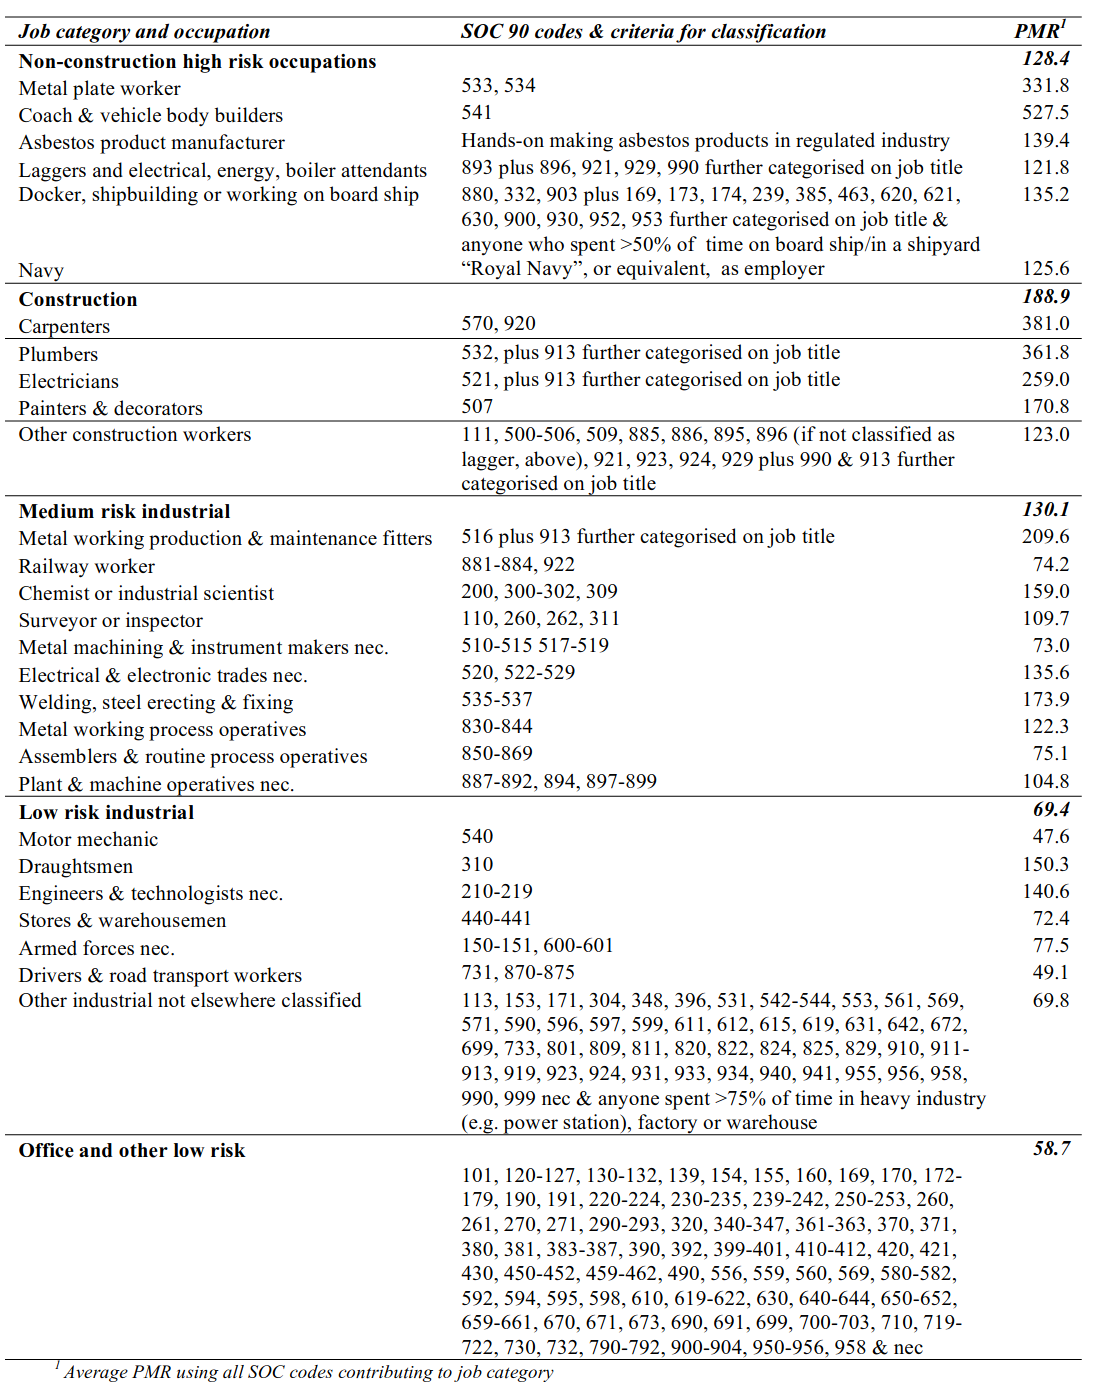
\includegraphics{source/figures/job_classification.png}
\caption{Classification of job categories with average national
mesothelioma PMRs. Table 2.3.2 in Occupational, domestic and
environmental mesothelioma risks in Britain. (HSE 2009)}
\end{figure}

For participants who recalled carrying out work with asbestos a detailed
assessment of each work task was recorded. A fibre-ml.year asbestos
exposure (AE) estimate was calculated using a source-receptor
model{[}@Cherrie1999{]}{[}@Cherrie2018{]}:

\begin{quote}
\ensuremath{AE = E \times H \times LC}
\end{quote}

with parameters for the type of asbestos used (substance emission
potential, E), what was done with it (activity emission potential, H),
how well ventilated the room the activity was carried out in was
(general ventilation parameters, D), and whether there were any local
exposure controls, for example wetting (local controls, LC).

AE for each task was then weighted according to the total amount of time
spent performing the task to arrive at a task fibre-ml.year exposure
estimate. Task fibre-ml.year exposure estimates were then summed at an
individual participant level to provide an overall fibre-ml.year
estimate. A random sample of high (top 25\% of values), medium (25-75\%
centile), and low (bottom 25\% of values) estimates was checked by a
hygiene assessment expert who was blind to participant case
status.{[}@Cherrie1999{]}{[}@Cherrie2018{]}

SOC90 coded jobs were also used to assign National Statistics
Socio-Economic analytic classes (NS-SEC). The Office of National
Statistics provides a lookup to assign each SOC90 code to one of eight
classes:

\begin{enumerate}
\def\labelenumi{\arabic{enumi}.}
\tightlist
\item
  Higher managerial, administrative and professional occupations. 1.1
  Large employers and higher managerial and administrative occupations.
  1.2 Higher professional occupations.
\item
  Lower managerial, administrative and professional occupations
\item
  Intermediate occupations
\item
  Small employers and own account workers
\item
  Lower supervisory and technical occupations
\item
  Semi-routine occupations
\item
  Routine occupations
\item
  Never worked and long-term unemployed
\end{enumerate}

We then assigned each individual to a single code by calculating the
median code for all of the jobs they had held.

Participants were classified as occupationally exposed to stone, wood,
and metal dust or not (binary measure) on the basis of the recorded
participant provided description of tasks carried out within a job
including the words `stone' (or `silica'), `wood', or `metal',
respectively.

All participants provided an EDTA sample from which DNA was extracted
and genotyped according to IPF known susceptibility SNP rs35705950. DNA
was extracted using a nucleon dna extraction kit. Genotypes of the MUC5B
SNP rs35705950 were determined using TaqMan assays (Life Technologies,
Carlsbad, CA). Reactions were performed in 96-well plates, and
fluorescence was read using an Applied Biosystems Viia7 Sequence
Detection System. See appendix 1 (or ipfjes.org) for full study protocol
including standard operating procedures.

\hypertarget{statistical-analysis}{%
\subsubsection{Statistical analysis}\label{statistical-analysis}}

Statistical analyses were carried out using Python{[}@van1995python{]},
SciPy{[}@2020SciPy-NMeth{]}, Statsmodels{[}@seabold2010statsmodels{]},
and Stata (StataCorp. 2015. Stata Statistical Software: Release 14.
College Station, TX: StataCorp LP).

For the primary analysis unconditional logistic regression was used to
analyse any vs no asbestos exposure and categories of cumulative
exposure adjusting for age and smoking status as part of a prespecified
analysis plan (clinicaltrials.gov NCT03211507). Prior data indicated
that the probability of exposure among controls is 0.63. If the true OR
for disease in exposed subjects relative to unexposed subjects is 1.5, I
calculated I would need to recruit 460 case patients and 460 control
patients to be able to reject the null hypothesis that this odds ratio
equals 1 with \ensuremath{\beta} = 0.2 and \ensuremath{\alpha} = 0.05;
my planned sample size included a margin for model stability and
incomplete data. In a planned secondary (exploratory) analysis I
investigated gene-environment interaction. The global minor allele
frequency of MUC5B rs35705950 is 0.05. With an estimated prevalence of
IPF of 20/100000 and with ORs 1.5 for asbestos exposure and 6.8 for
rs35705950, 460 cases would be required to detect a minimum interaction
OR of 5.0.

In an unplanned secondary analyses I used logistic regression to
investigate metal, wood, and stone dust exposure (self-reported
occupational exposure), and rs35705950 genotype-exposure interactions.
Sensitivity analysis of distance to centre was also performed because I
expected cases to live further away from the hospital that controls on
average (as IPF care is centralised to a select number of specialist
centres) and I hypothesised that distance from the hospital might be
associated with likelihood of exposure to asbestos. I used Pearson's
correlation coefficient to investigate associations between individual
variables, such as distance from hospital and fibre-ml.year asbestos
exposure estimates. I used ordinal logistic regression to investigate
the relationship between mMRC dyspnoea score and measures of asbestos
exposure.

In the course of this work I learned that the minor allele of rs35705950
was associated with asbestosis{[}@Platenburg2020{]}, that smoking and
asbestos exposure interact significantly in
asbestosis{[}@Mossman1998{]}, and that this interaction is likely to be
mediated by NLRP3 inflammasome activation{[}@Dostert2008{]}; a process
which results in increased MUC5b expression. This led me to hypothesise
that there may be an interaction between rs35705950, asbestos, and
smoking. To test this hypothesis I stratified by genotype and
investigated interactions between smoking and occupational asbestos
exposure using unconditional logistic regression.

\hypertarget{results}{%
\subsection{Results}\label{results}}

Five hundred and sixteen cases and 511 controls were recruited to IPFJES
in the study period Feb 2017 to October 2019. Twenty two cases(4\%), and
45 of 511 controls(9\%) were withdrawn because they no longer wished to
take part in the study, they did not respond after we called them on
three occasions, or we were notified that they had died before the
interview took place. The remaining 960 participants (494 cases, 466
controls) comprise the study sample.

The median year of birth and age was 1943 and 76 for cases and 1945 and
74 for controls. Most cases and controls reported their ethnicity as
white (97\% and 96\% respectively). Social economic class and exposure
to smoking were similar for cases and controls (see Table 6.1).

\newpage

\hypertarget{table-6.1-participant-demographic-characteristics}{%
\subsubsection{Table 6.1: Participant demographic
characteristics}\label{table-6.1-participant-demographic-characteristics}}

\begin{longtable}[]{@{}lllll@{}}
\toprule
Characteristic & Cases (N=494) & \% & Controls (N=466) &
\%\tabularnewline
\midrule
\endhead
Age -- yr & & & &\tabularnewline
median & 76 & & 74 &\tabularnewline
interquartile range & 71-81 & & 69-79 &\tabularnewline
& & & &\tabularnewline
Ethnicity & & & &\tabularnewline
White & 479 & 97 & 449 & 96\tabularnewline
Asian/Asian British & 11 & 2 & 8 & 2\tabularnewline
Black/African & 2 & 0 & 7 & 2\tabularnewline
Mixed/Other & 2 & 0 & 2 & 0\tabularnewline
& & & &\tabularnewline
Social class & & & &\tabularnewline
1.1 & 2 & 0 & 11 & 2\tabularnewline
1.2 & 33 & 7 & 28 & 6\tabularnewline
2 & 58 & 12 & 63 & 14\tabularnewline
3 & 73 & 15 & 71 & 15\tabularnewline
4 & 53 & 11 & 50 & 11\tabularnewline
5 & 92 & 19 & 100 & 21\tabularnewline
6 & 117 & 24 & 87 & 19\tabularnewline
7 & 66 & 13 & 56 & 12\tabularnewline
& & & &\tabularnewline
Smoking & & & &\tabularnewline
Current smoker & 10 & 2 & 30 & 6\tabularnewline
Ever smoked & 373 & 76 & 327 & 70\tabularnewline
Packyears & & & &\tabularnewline
mean & 27 & & 24 &\tabularnewline
median & 20 & & 19 &\tabularnewline
interquartile range & 9-36 & & 7-34 &\tabularnewline
\bottomrule
\end{longtable}

All cases had a CT thorax and this was reported as showing definite UIP
in 266 (54\%) cases, possible UIP in 216 (44\%) cases, or `other' in 12
(2\%) cases. Nine cases (2\%) had a biopsy because the CT was
non-diagnostic; all of these were reported as definite UIP. Cases were
more breathless than controls as measured by the Medical Research
Council (MRC) dyspnoea scale. Known rs3570950 IPF associations were
evident (see Table 6.2).

\hypertarget{table-6.2-patient-clinical-features-from-case-report-form-and-genotypes}{%
\subsubsection{Table 6.2: Patient clinical features (from case report
form) and
genotypes}\label{table-6.2-patient-clinical-features-from-case-report-form-and-genotypes}}

\begin{longtable}[]{@{}lllll@{}}
\toprule
& Cases (N=494) & \% & Controls (N=466) & \%\tabularnewline
\midrule
\endhead
CT & & & &\tabularnewline
no CT & 0 & 0 & 462 & 99\tabularnewline
definite UIP & 266 & 54 & 1\textsuperscript{1} & 0\tabularnewline
possible UIP & 216 & 44 & 0 & 0\tabularnewline
other & 12 & 2 & 3 & 1\tabularnewline
& & & &\tabularnewline
Bx & & & &\tabularnewline
no biopsy & 485 & 98 & 466 & 100\tabularnewline
definite UIP & 9 & 2 & 0 & 0\tabularnewline
& & & &\tabularnewline
mMRC & & & &\tabularnewline
0 & 35 & 7 & 254 & 55\tabularnewline
1 & 94 & 19 & 65 & 14\tabularnewline
2 & 165 & 33 & 80 & 17\tabularnewline
3 & 172 & 35 & 65 & 14\tabularnewline
4 & 28 & 6 & 2 & 0\tabularnewline
& & & &\tabularnewline
rs35705950 genotype & N=395 & & N=423 &\tabularnewline
(G;G) & 152 & 38 & 327 & 77\tabularnewline
(G;T) & 212 & 54 & 91 & 22\tabularnewline
(T;T) & 31 & 8 & 5 & 1\tabularnewline
\bottomrule
\end{longtable}

\textsuperscript{1} one control had rheumatoid arthritis associated
interstitial lung disease

Recruiting centres were geographically dispersed across England,
Scotland, and Wales. See Figure 6.2.

\begin{figure}
\centering
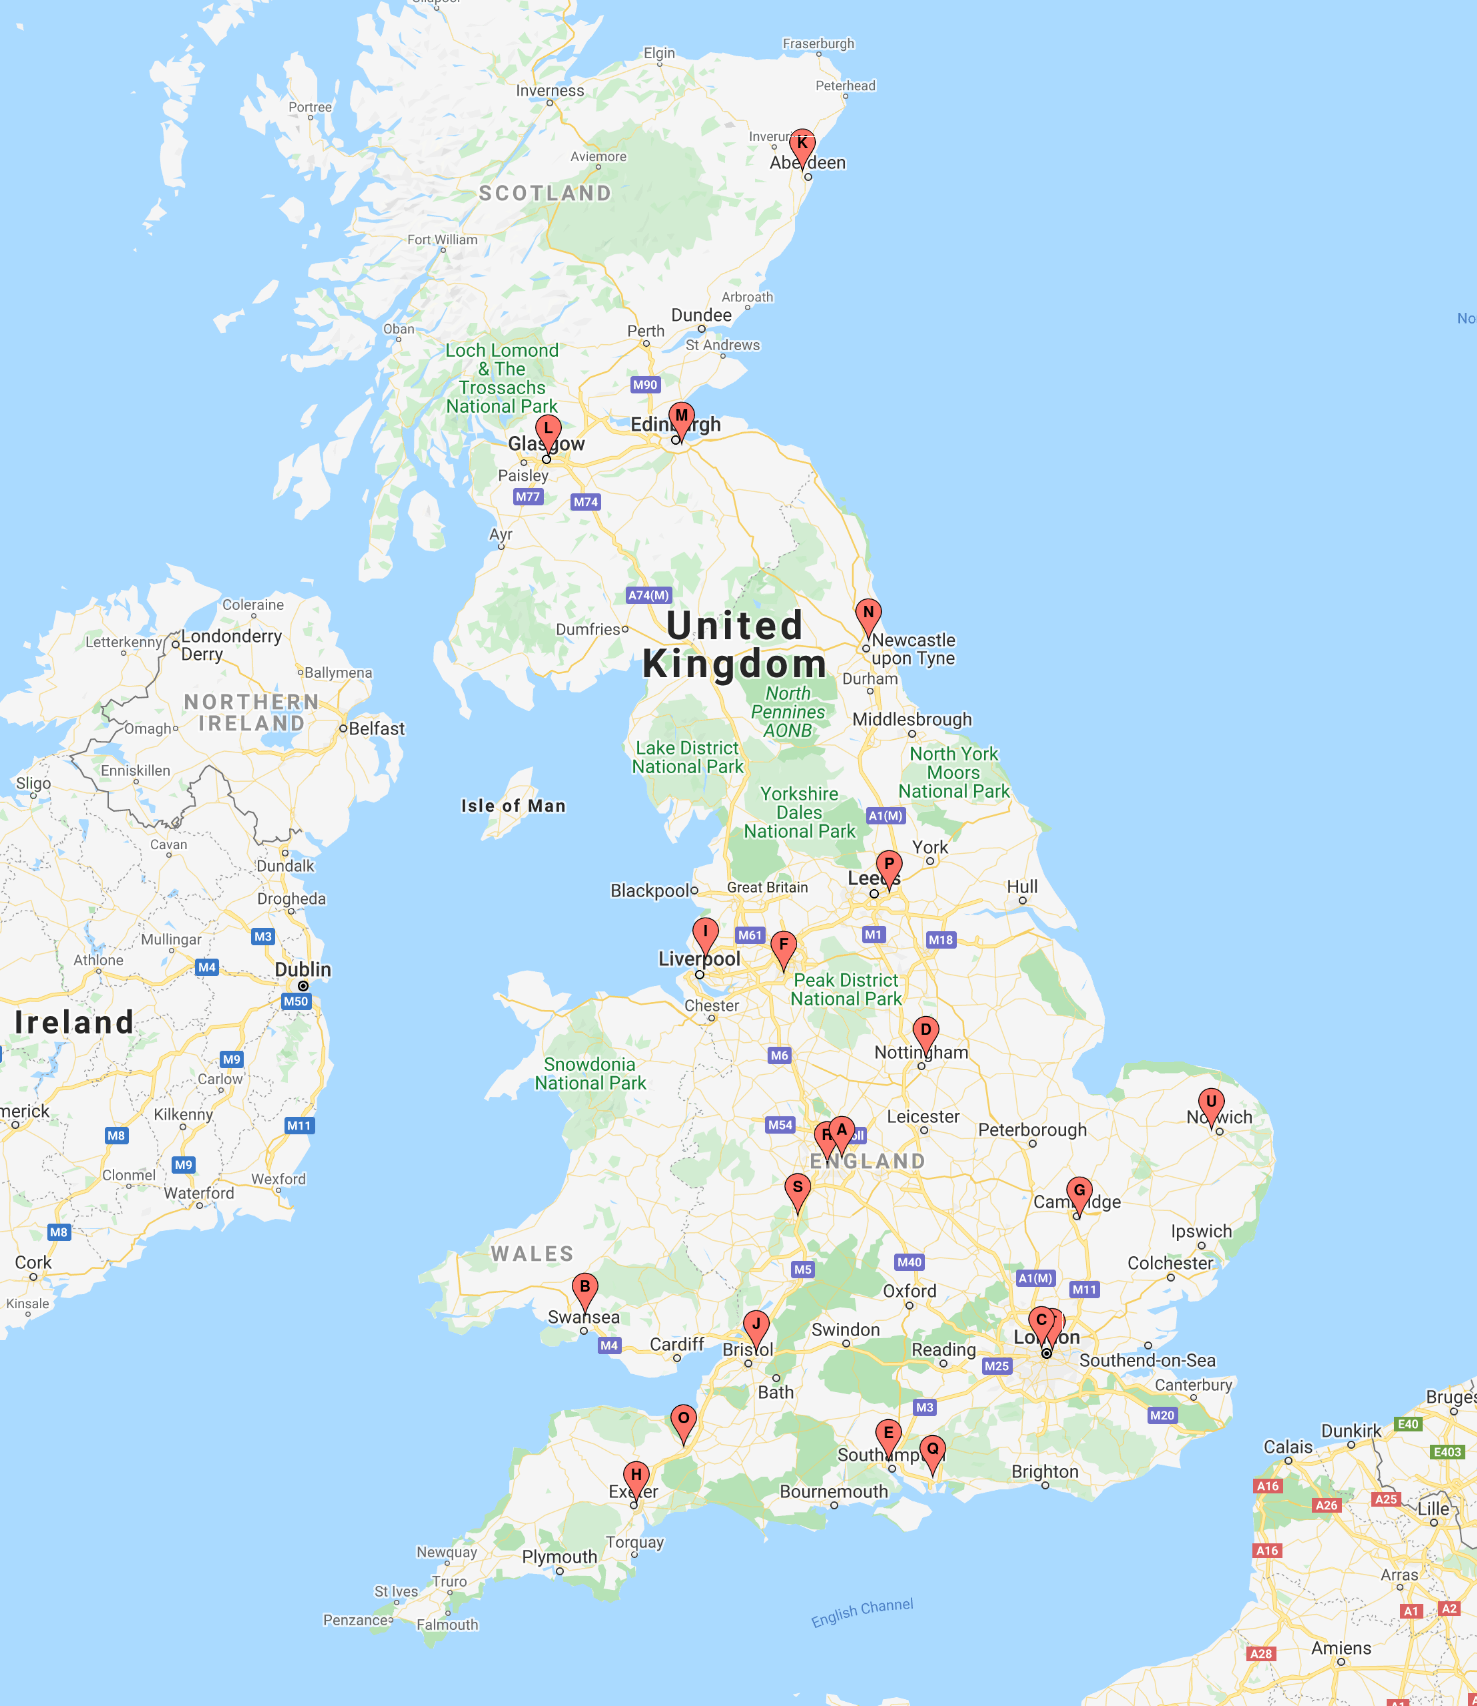
\includegraphics{source/figures/ipfjes_centres.png}
\caption{Map showing the 21 IPFJES recruiting centres
\label{ipfjescentres}}
\end{figure}

Randomly selected control clinics for recruiting centres are shown in
Table 6.3. Where more than one clinic is shown this indicates that the
random selection process was repeated because of difficulty recruiting
adequate numbers of participants (defined as four attendances to the
control clinic by the local research team and fewer than four
participants recruited).

\newpage

\hypertarget{table-6.3-centre-control-clinics-and-recruitment}{%
\subsubsection{Table 6.3: Centre control clinics and
recruitment}\label{table-6.3-centre-control-clinics-and-recruitment}}

\begin{longtable}[]{@{}lll@{}}
\toprule
& Cases (N=494) & Controls (N=466)\tabularnewline
\midrule
\endhead
centre number (control source clinic) & &\tabularnewline
1 (General Surgery) & 42 & 39\tabularnewline
2 (Gastroenterology/Stroke)\textsuperscript{1} & 13 & 11\tabularnewline
3 (Cardiology) & 38 & 36\tabularnewline
4 (Urology) & 52 & 52\tabularnewline
5 (Diabetes/Rheumatology)\textsuperscript{1} & 40 & 31\tabularnewline
6 (Sleep Apnoea) & 34 & 37\tabularnewline
7 (Neurology) & 15 & 16\tabularnewline
8 (ENT) & 40 & 39\tabularnewline
9 (Rheumatology) & 31 & 29\tabularnewline
10 (Oncology) & 21 & 73\textsuperscript{2}\tabularnewline
11 (Urology) & 11 & 11\tabularnewline
12 (Haematology) & 4 & 3\tabularnewline
13 (Respiratory) & 13 & 14\tabularnewline
14 (Cardiology) & 20 & 16\tabularnewline
15 (Cardiology) & 15 & 14\tabularnewline
16 (Orthopaedics) & 39 & 2\textsuperscript{3}\tabularnewline
17 (Asthma) & 6 & 6\tabularnewline
18 (Hypertension) & 15 & 1\textsuperscript{3}\tabularnewline
19 (General Surgery) & 7 & 9\tabularnewline
20 (Urology) & 31 & 25\tabularnewline
21 (Respiratory) & 7 & 2\tabularnewline
\bottomrule
\end{longtable}

\textsuperscript{1} The control clinic changed at these two sites
because of slow recruitment (defined as fewer than four controls
recruited over the course of four clinic attendances).
\textsuperscript{2} Controls were over-recruited at the local
participating centre to help achieve the recruitment target.
\textsuperscript{3} Controls were under-recruited because of local
research staffing shortage.

Three hundred and thirty (67\%) cases and 295 (63\%) controls ever had a
high or medium asbestos exposure risk job, defined on the basis of
proportional occupational mortality statistics.{[}@Peto2009{]} Ever
having a high or medium asbestos exposure risk job was not associated
with IPF (see Table 6.4).

\hypertarget{table-6.4-occupational-asbestos-exposure-inferred-by-job-title-and-ipf-risk-ever-vs-never}{%
\subsubsection{Table 6.4: Occupational asbestos exposure (inferred by
job title) and IPF risk (ever vs
never)}\label{table-6.4-occupational-asbestos-exposure-inferred-by-job-title-and-ipf-risk-ever-vs-never}}

\begin{longtable}[]{@{}lllll@{}}
\toprule
\begin{minipage}[b]{0.06\columnwidth}\raggedright
\strut
\end{minipage} & \begin{minipage}[b]{0.10\columnwidth}\raggedright
Cases (\%)\strut
\end{minipage} & \begin{minipage}[b]{0.12\columnwidth}\raggedright
Controls (\%)\strut
\end{minipage} & \begin{minipage}[b]{0.29\columnwidth}\raggedright
Unadjusted OR (95\%CI; p-value)\strut
\end{minipage} & \begin{minipage}[b]{0.28\columnwidth}\raggedright
Adjusted OR\textsuperscript{1} (95\%CI; p-value)\strut
\end{minipage}\tabularnewline
\midrule
\endhead
\begin{minipage}[t]{0.06\columnwidth}\raggedright
ever\strut
\end{minipage} & \begin{minipage}[t]{0.10\columnwidth}\raggedright
330(67)\strut
\end{minipage} & \begin{minipage}[t]{0.12\columnwidth}\raggedright
295(63)\strut
\end{minipage} & \begin{minipage}[t]{0.29\columnwidth}\raggedright
1.17(0.9-1.5; 0.28)\strut
\end{minipage} & \begin{minipage}[t]{0.28\columnwidth}\raggedright
1.09(0.8-1.5; 0.6)\strut
\end{minipage}\tabularnewline
\bottomrule
\end{longtable}

1 \textbar{} 1 \textbar{}

\textsuperscript{1} Adjusted for age, smoking, and centre

There was a non-statistically significant trend in the unadjusted OR
whereby higher exposure categories had higher (non-significant) ORs for
disease (see Table 6.5). This was less apparent in adjusted analyses
(chi\textsuperscript{2} test for trend was 1.7, p=0.19).

\newpage

\hypertarget{table-6.5-occupational-asbestos-exposure-inferred-by-job-title-and-ipf-risk-categories-of-exposure}{%
\subsubsection{Table 6.5: Occupational asbestos exposure (inferred by
job title) and IPF risk (categories of
exposure)}\label{table-6.5-occupational-asbestos-exposure-inferred-by-job-title-and-ipf-risk-categories-of-exposure}}

\begin{longtable}[]{@{}lllll@{}}
\toprule
\begin{minipage}[b]{0.20\columnwidth}\raggedright
Category\strut
\end{minipage} & \begin{minipage}[b]{0.08\columnwidth}\raggedright
Cases (\%)\strut
\end{minipage} & \begin{minipage}[b]{0.10\columnwidth}\raggedright
Controls (\%)\strut
\end{minipage} & \begin{minipage}[b]{0.24\columnwidth}\raggedright
Unadjusted OR (95\%CI; p-value)\strut
\end{minipage} & \begin{minipage}[b]{0.23\columnwidth}\raggedright
Adjusted OR\textsuperscript{1} (95\%CI; p-value)\strut
\end{minipage}\tabularnewline
\midrule
\endhead
\begin{minipage}[t]{0.20\columnwidth}\raggedright
high-risk non-construction\strut
\end{minipage} & \begin{minipage}[t]{0.08\columnwidth}\raggedright
65(13)\strut
\end{minipage} & \begin{minipage}[t]{0.10\columnwidth}\raggedright
52(11)\strut
\end{minipage} & \begin{minipage}[t]{0.24\columnwidth}\raggedright
1.30(0.8-2.1;0.3)\strut
\end{minipage} & \begin{minipage}[t]{0.23\columnwidth}\raggedright
1.10(0.7-1.8; 0.7)\strut
\end{minipage}\tabularnewline
\begin{minipage}[t]{0.20\columnwidth}\raggedright
high-risk construction\strut
\end{minipage} & \begin{minipage}[t]{0.08\columnwidth}\raggedright
141(29)\strut
\end{minipage} & \begin{minipage}[t]{0.10\columnwidth}\raggedright
126(27)\strut
\end{minipage} & \begin{minipage}[t]{0.24\columnwidth}\raggedright
1.17(0.8-1.8;0.5)\strut
\end{minipage} & \begin{minipage}[t]{0.23\columnwidth}\raggedright
1.13(0.8-1.7; 0.55)\strut
\end{minipage}\tabularnewline
\begin{minipage}[t]{0.20\columnwidth}\raggedright
medium risk industrial\strut
\end{minipage} & \begin{minipage}[t]{0.08\columnwidth}\raggedright
124(25)\strut
\end{minipage} & \begin{minipage}[t]{0.10\columnwidth}\raggedright
117(25)\strut
\end{minipage} & \begin{minipage}[t]{0.24\columnwidth}\raggedright
1.11(0.7-1.7;0.64)\strut
\end{minipage} & \begin{minipage}[t]{0.23\columnwidth}\raggedright
1.06(0.7-1.6; 0.79)\strut
\end{minipage}\tabularnewline
\begin{minipage}[t]{0.20\columnwidth}\raggedright
low risk industrial\strut
\end{minipage} & \begin{minipage}[t]{0.08\columnwidth}\raggedright
94(19)\strut
\end{minipage} & \begin{minipage}[t]{0.10\columnwidth}\raggedright
98(21)\strut
\end{minipage} & \begin{minipage}[t]{0.24\columnwidth}\raggedright
1(0.7-1.5;0.99)\strut
\end{minipage} & \begin{minipage}[t]{0.23\columnwidth}\raggedright
0.94(0.6-1.5; 0.78)\strut
\end{minipage}\tabularnewline
\begin{minipage}[t]{0.20\columnwidth}\raggedright
office\strut
\end{minipage} & \begin{minipage}[t]{0.08\columnwidth}\raggedright
70(14)\strut
\end{minipage} & \begin{minipage}[t]{0.10\columnwidth}\raggedright
73(16)\strut
\end{minipage} & \begin{minipage}[t]{0.24\columnwidth}\raggedright
1\strut
\end{minipage} & \begin{minipage}[t]{0.23\columnwidth}\raggedright
1\strut
\end{minipage}\tabularnewline
\bottomrule
\end{longtable}

\textsuperscript{1} Adjusted for age, smoking, and centre

A total of 463 asbestos exposed job tasks were recalled in sufficient
detail to permit a fibre-ml.year estimate of exposure for 233 individual
participants. One hundred and twenty five (25\%) of cases and 108 (23\%)
controls recalled occupational asbestos exposure in sufficient detail to
permit estimation of cumulative fibre-ml.year exposure. Forty one (33\%)
cases and 35 (32\%) controls, which equated to approximately 8\% of the
total number of cases and 8\% of the total number of controls, had
cumulative estimates exceeding 25 asbestos fibre-ml.years (see Table
6.6).

Fibre-ml.year exposure assessments showed reasonable correlation on the
log-scale, but not the linear scale, with an independent assessor (JC)
for a validation sample of low, medium, and high exposure assessments,
R\textsuperscript{2} = 0.63 (see Figure 6.3).

\begin{figure}
\centering
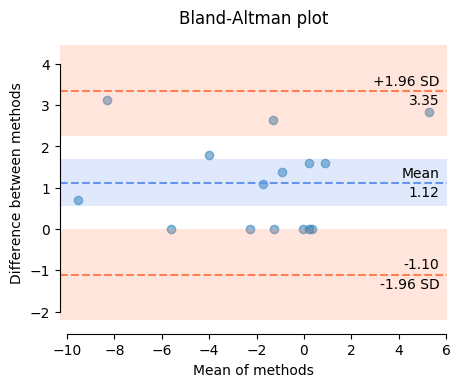
\includegraphics{source/figures/cherrie_validation.png}
\caption{Independent validation of fibre-ml.year exposure assessments}
\end{figure}

\newpage

\hypertarget{table-6.6-occupational-asbestos-exposure-cumulative-fibre-ml-year-estimate-and-ipf-risk}{%
\subsubsection{Table 6.6: Occupational asbestos exposure (cumulative
fibre ml year estimate) and IPF
risk}\label{table-6.6-occupational-asbestos-exposure-cumulative-fibre-ml-year-estimate-and-ipf-risk}}

\begin{longtable}[]{@{}lllllllll@{}}
\toprule
& N (\% total) & median & 0-4 & 5-9 & 10-14 & 15-19 & 20-24 &
\textgreater{} 25\tabularnewline
\midrule
\endhead
cases & 125 (25) & 6.86 & 62 (50) & 10 (8) & 5 (4) & 3 (2) & 4 (3) & 41
(33)\tabularnewline
controls & 108 (23) & 4.36 & 56 (52) & 4 (4) & 8 (7) & 0 (0) & 5 (5) &
35 (32)\tabularnewline
\bottomrule
\end{longtable}

One hundred and eight (23\%) of the 463 asbestos exposed job task
fibre-ml.year estimates were in excess of 25 fibre-ml.years. Eighty one
(75\%) occurred in jobs classified as high risk or medium risk; 17(15\%)
occurred in high-risk non-construction jobs e.g boiler lagger, 54(50\%)
in high-risk construction jobs such as carpenter, electrician, and
plumber, and 10 (9\%) in medium risk industrial jobs such as machinist
or fitter. Carpenter was the single most common job title accounting for
6(5\%) of estimates in excess of 25 fibre-ml.years (see Figures 6.4 and
6.5).

\begin{figure}
\centering
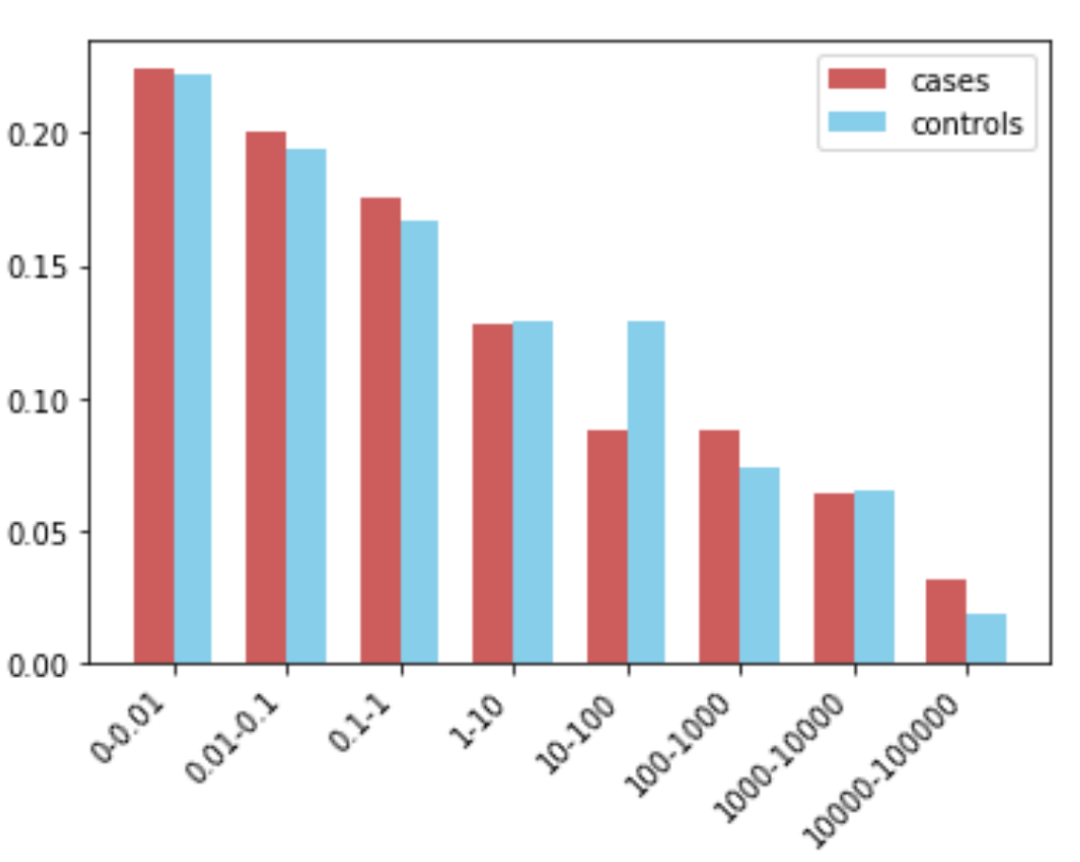
\includegraphics{source/figures/fibre.png}
\caption{Proportion of exposed participants in fibre-ml.year categories
of exposure for those reporting exposure (N=233)}
\end{figure}

\begin{figure}
\centering
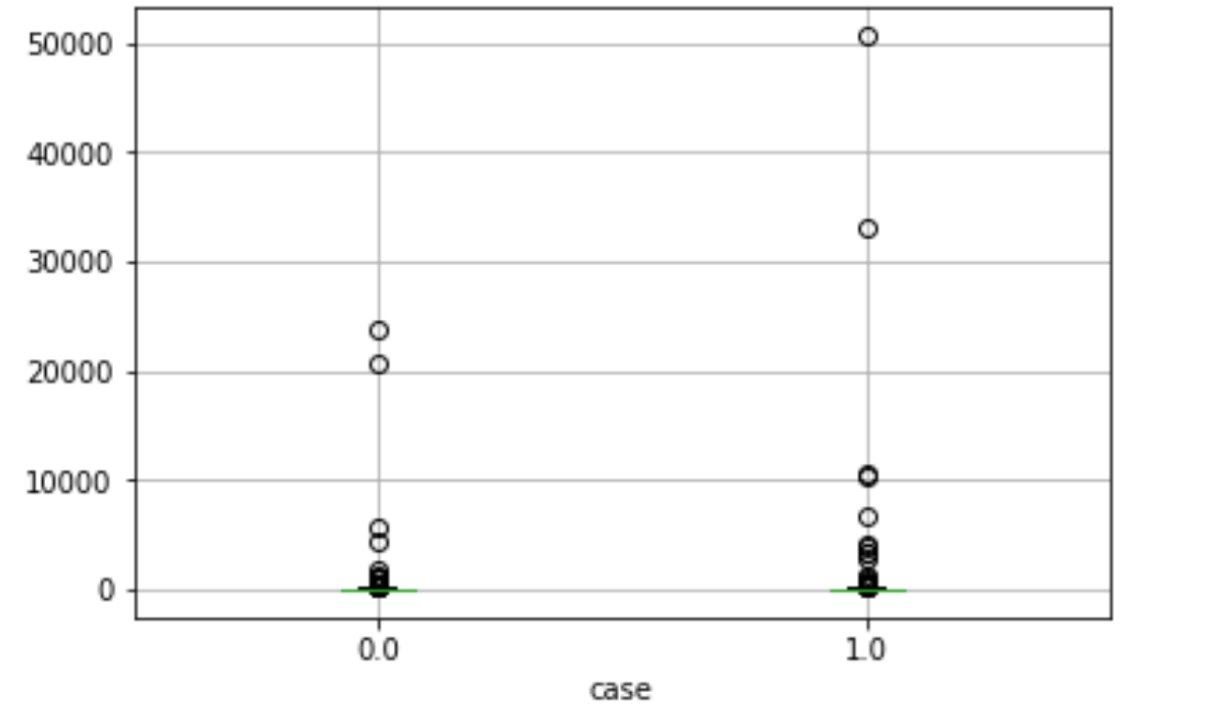
\includegraphics{source/figures/fibre2.png}
\caption{Boxplot of fibre-ml.year asbestos exposure estimates for cases
and controls for those reporting exposure (N=233)}
\end{figure}

Eight hundred and eighteen (85\%) of the 960 participants were genotyped
for MUC5b rs3570950. Ninety participant samples remain to be genotyped
(because of staffing issues) while 52 participants did not provide a
sample. Being heterozygous for the disease associated variant (GT) had
an odds ratio of 5 (95\%CI 3.7-6.8; p \ensuremath{<} 0.001) for disease.
Being homozygous for the disease associated variant (TT) had an odds
ratio of 13.3 (95\%CI 5.1-35, p \ensuremath{<} 0.001) for disease. Ever
having smoked was associated with an increased risk of disease, odds
ratio 1.4 (95\%CI 1-1.8, p \ensuremath{<} 0.03). There was a
statistically significant interaction between smoking and having ever
been exposed to a high or medium asbestos exposure risk job, odds ratio
for interaction 1.9 (95\%CI 1.03-3.36, p \ensuremath{<} 0.04). Several
non-significant gene-environment interactions were present (see Table
6.7).

\hypertarget{table-6.7-muc5b-rs35705950-occupational-asbestos-exposure-smoking-and-ipf-risk}{%
\subsubsection{Table 6.7: MUC5b rs35705950, occupational asbestos
exposure, smoking, and IPF
risk}\label{table-6.7-muc5b-rs35705950-occupational-asbestos-exposure-smoking-and-ipf-risk}}

\begin{longtable}[]{@{}ll@{}}
\toprule
Exposure & OR (95\%CI; p-value)\textsuperscript{1}
\textsuperscript{2}\tabularnewline
\midrule
\endhead
rs35705950 &\tabularnewline
GG & 1\tabularnewline
GT & 5 (3.7-6.8; \ensuremath{<} 0.001)\tabularnewline
TT & 13.3 (5.1-35; \ensuremath{<} 0.001)\tabularnewline
&\tabularnewline
Ever smoked & 1.4 (1-1.8; 0.03)\textsuperscript{3}\tabularnewline
EE interaction (smoking and ever exposed) & 1.9 (1.03-3.36;
0.04)\textsuperscript{3}\tabularnewline
&\tabularnewline
GE interaction (ever exposed) & 1.5 (0.8-2.7; 0.2)\tabularnewline
GE interaction (categories of exposure) & 1.1(0.9-1.4;
0.38)\tabularnewline
GE interaction (fibre-ml years) & 1(0.99-1; 0.34)\tabularnewline
GE interaction (ever smoked) & 1.2 (0.6-2.2; 0.7)\tabularnewline
\bottomrule
\end{longtable}

\textsuperscript{1} additive model, adjusted for age and smoking, N=818
for analysis involving genotype and N=960 for analysis not involving
genotype\\
\textsuperscript{2} adjusted for age only where smoking is exposure\\
\textsuperscript{3} when adjusting for centre also, ever smoked remains
significant but smoking and ever exposed does not

The regression coefficient for MUC5b rs35705950 genotype, using an
additive model, was significant but age, smoking, asbestos exposure, and
the interaction of asbestos exposure and genotype were not. See
dot-and-whisker plot of regression coefficients (Figure 6.6).

\begin{figure}
\centering
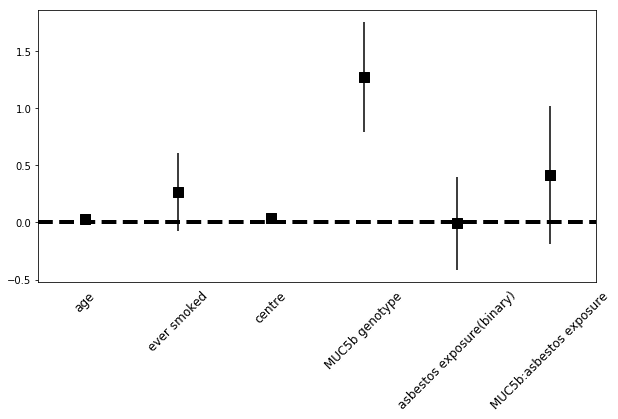
\includegraphics{source/figures/regression_coefficients.png}
\caption{Regression coefficients (and 95\% confidence intervals) for
logistic regression of case status against age in years, ever having
smoked (binary), centre, MUC5b rs35705950 genotype (additive model),
asbestos exposure (ever held high or medium risk asbestos exposure job
based on job title), and gene-environment interaction (N=818)}
\end{figure}

Ever having a job with wood, metal, or stone exposure was associated
with disease, odds ratio 1.7 (95\%CI 1.2-2.3, p \ensuremath{<} 0.01).
Stone dust exposure alone was associated with a statistically
significant odds ratio for disease of 2.9 (95\%CI 1.3-6.7, p
\ensuremath{<} 0.01) but wood and metal dust were not (see Table 6.8).

\hypertarget{table-6.8-occupational-metal-wood-and-stone-exposure-and-ipf-risk}{%
\subsubsection{Table 6.8: Occupational metal, wood, and stone exposure
and IPF
risk}\label{table-6.8-occupational-metal-wood-and-stone-exposure-and-ipf-risk}}

\begin{longtable}[]{@{}lllll@{}}
\toprule
\begin{minipage}[b]{0.20\columnwidth}\raggedright
Exposure\strut
\end{minipage} & \begin{minipage}[b]{0.08\columnwidth}\raggedright
Cases (\%)\strut
\end{minipage} & \begin{minipage}[b]{0.10\columnwidth}\raggedright
Controls (\%)\strut
\end{minipage} & \begin{minipage}[b]{0.24\columnwidth}\raggedright
Unadjusted OR (95\%CI; p-value)\strut
\end{minipage} & \begin{minipage}[b]{0.24\columnwidth}\raggedright
Adjusted OR\textsuperscript{1} (95\%CI; p-value)\strut
\end{minipage}\tabularnewline
\midrule
\endhead
\begin{minipage}[t]{0.20\columnwidth}\raggedright
Wood, metal, stone (any)\strut
\end{minipage} & \begin{minipage}[t]{0.08\columnwidth}\raggedright
139(28)\strut
\end{minipage} & \begin{minipage}[t]{0.10\columnwidth}\raggedright
84(18)\strut
\end{minipage} & \begin{minipage}[t]{0.24\columnwidth}\raggedright
1.8(1.3-2.4; \ensuremath{<}0.01)\strut
\end{minipage} & \begin{minipage}[t]{0.24\columnwidth}\raggedright
1.7(1.2-2.3; \ensuremath{<}0.01)\strut
\end{minipage}\tabularnewline
\begin{minipage}[t]{0.20\columnwidth}\raggedright
Wood\strut
\end{minipage} & \begin{minipage}[t]{0.08\columnwidth}\raggedright
48(10)\strut
\end{minipage} & \begin{minipage}[t]{0.10\columnwidth}\raggedright
31(7)\strut
\end{minipage} & \begin{minipage}[t]{0.24\columnwidth}\raggedright
1.5(0.9-2.4; 0.09)\strut
\end{minipage} & \begin{minipage}[t]{0.24\columnwidth}\raggedright
1.4(0.9-2.3; 0.2)\strut
\end{minipage}\tabularnewline
\begin{minipage}[t]{0.20\columnwidth}\raggedright
Metal\strut
\end{minipage} & \begin{minipage}[t]{0.08\columnwidth}\raggedright
88(18)\strut
\end{minipage} & \begin{minipage}[t]{0.10\columnwidth}\raggedright
57(12)\strut
\end{minipage} & \begin{minipage}[t]{0.24\columnwidth}\raggedright
1.6(1.1-2.2; 0.02)\strut
\end{minipage} & \begin{minipage}[t]{0.24\columnwidth}\raggedright
1.4(0.9-2.0; 0.1)\strut
\end{minipage}\tabularnewline
\begin{minipage}[t]{0.20\columnwidth}\raggedright
Stone\strut
\end{minipage} & \begin{minipage}[t]{0.08\columnwidth}\raggedright
24(5)\strut
\end{minipage} & \begin{minipage}[t]{0.10\columnwidth}\raggedright
8(2)\strut
\end{minipage} & \begin{minipage}[t]{0.24\columnwidth}\raggedright
2.9(1.3-6.6; 0.01)\strut
\end{minipage} & \begin{minipage}[t]{0.24\columnwidth}\raggedright
2.9(1.3-6.7; 0.01)\strut
\end{minipage}\tabularnewline
\bottomrule
\end{longtable}

\textsuperscript{1} Adjusted for age, smoking, and centre

As a result of increasing awareness, and regulation, occupational
asbestos exposure was significantly less widespread after
1980.{[}@Gilham2018{]} To investigate whether occupational asbestos
exposure might be associated with IPF during this period I performed a
sensitivity analysis by only including participants jobs that ended
before 1980. I did not observe a significant association (Table 6.9 and
6.10). I also performed sensitivity analyses limiting to jobs that
started before 1980, participants born prior to 1965, and considering
only jobs before age 45{[}@Darnton2012{]}; there was no significant
association between asbestos exposure and IPF for these.

\newpage

\hypertarget{table-6.9-sensitivity-analysis-limited-to-jobs-that-ended-before-1980-occupational-asbestos-exposure-inferred-by-job-title-and-ipf-risk-ever-vs-never}{%
\subsubsection{Table 6.9: Sensitivity analysis (limited to jobs that
ended before 1980): Occupational asbestos exposure (inferred by job
title) and IPF risk (ever vs
never)}\label{table-6.9-sensitivity-analysis-limited-to-jobs-that-ended-before-1980-occupational-asbestos-exposure-inferred-by-job-title-and-ipf-risk-ever-vs-never}}

\begin{longtable}[]{@{}lllll@{}}
\toprule
\begin{minipage}[b]{0.06\columnwidth}\raggedright
\strut
\end{minipage} & \begin{minipage}[b]{0.10\columnwidth}\raggedright
Cases (\%)\strut
\end{minipage} & \begin{minipage}[b]{0.12\columnwidth}\raggedright
Controls (\%)\strut
\end{minipage} & \begin{minipage}[b]{0.29\columnwidth}\raggedright
Unadjusted OR (95\%CI; p-value)\strut
\end{minipage} & \begin{minipage}[b]{0.28\columnwidth}\raggedright
Adjusted OR\textsuperscript{1} (95\%CI; p-value)\strut
\end{minipage}\tabularnewline
\midrule
\endhead
\begin{minipage}[t]{0.06\columnwidth}\raggedright
ever\strut
\end{minipage} & \begin{minipage}[t]{0.10\columnwidth}\raggedright
250(62)\strut
\end{minipage} & \begin{minipage}[t]{0.12\columnwidth}\raggedright
220(59)\strut
\end{minipage} & \begin{minipage}[t]{0.29\columnwidth}\raggedright
1.11(0.8-1.5; 0.46)\strut
\end{minipage} & \begin{minipage}[t]{0.28\columnwidth}\raggedright
0.97(0.72-1.32; 0.87)\strut
\end{minipage}\tabularnewline
\begin{minipage}[t]{0.06\columnwidth}\raggedright
never\strut
\end{minipage} & \begin{minipage}[t]{0.10\columnwidth}\raggedright
156(38)\strut
\end{minipage} & \begin{minipage}[t]{0.12\columnwidth}\raggedright
153(41)\strut
\end{minipage} & \begin{minipage}[t]{0.29\columnwidth}\raggedright
1\strut
\end{minipage} & \begin{minipage}[t]{0.28\columnwidth}\raggedright
1\strut
\end{minipage}\tabularnewline
\bottomrule
\end{longtable}

\textsuperscript{1} Adjusted for age, smoking, and centre

\hypertarget{table-6.10-sensitivity-analysis-limited-to-jobs-that-ended-before-1980-occupational-asbestos-exposure-inferred-by-job-title-and-ipf-risk-categories-of-exposure}{%
\subsubsection{Table 6.10: Sensitivity analysis (limited to jobs that
ended before 1980): Occupational asbestos exposure (inferred by job
title) and IPF risk (categories of
exposure)}\label{table-6.10-sensitivity-analysis-limited-to-jobs-that-ended-before-1980-occupational-asbestos-exposure-inferred-by-job-title-and-ipf-risk-categories-of-exposure}}

\begin{longtable}[]{@{}lllll@{}}
\toprule
\begin{minipage}[b]{0.20\columnwidth}\raggedright
Category\strut
\end{minipage} & \begin{minipage}[b]{0.08\columnwidth}\raggedright
Cases (\%)\strut
\end{minipage} & \begin{minipage}[b]{0.10\columnwidth}\raggedright
Controls (\%)\strut
\end{minipage} & \begin{minipage}[b]{0.24\columnwidth}\raggedright
Unadjusted OR (95\%CI; p-value)\strut
\end{minipage} & \begin{minipage}[b]{0.23\columnwidth}\raggedright
Adjusted OR\textsuperscript{1} (95\%CI; p-value)\strut
\end{minipage}\tabularnewline
\midrule
\endhead
\begin{minipage}[t]{0.20\columnwidth}\raggedright
high-risk non-construction\strut
\end{minipage} & \begin{minipage}[t]{0.08\columnwidth}\raggedright
53(13)\strut
\end{minipage} & \begin{minipage}[t]{0.10\columnwidth}\raggedright
36(10)\strut
\end{minipage} & \begin{minipage}[t]{0.24\columnwidth}\raggedright
1.55(0.9-2.6;0.62)\strut
\end{minipage} & \begin{minipage}[t]{0.23\columnwidth}\raggedright
1.09(0.61-1.94;0.77)\strut
\end{minipage}\tabularnewline
\begin{minipage}[t]{0.20\columnwidth}\raggedright
high-risk construction\strut
\end{minipage} & \begin{minipage}[t]{0.08\columnwidth}\raggedright
95(23)\strut
\end{minipage} & \begin{minipage}[t]{0.10\columnwidth}\raggedright
81(22)\strut
\end{minipage} & \begin{minipage}[t]{0.24\columnwidth}\raggedright
1.22(0.8-1.9;0.88)\strut
\end{minipage} & \begin{minipage}[t]{0.23\columnwidth}\raggedright
1.01(0.63-1.63;0.97)\strut
\end{minipage}\tabularnewline
\begin{minipage}[t]{0.20\columnwidth}\raggedright
medium risk industrial\strut
\end{minipage} & \begin{minipage}[t]{0.08\columnwidth}\raggedright
102(25)\strut
\end{minipage} & \begin{minipage}[t]{0.10\columnwidth}\raggedright
103(28)\strut
\end{minipage} & \begin{minipage}[t]{0.24\columnwidth}\raggedright
1.03(0.7-1.6;0.37)\strut
\end{minipage} & \begin{minipage}[t]{0.23\columnwidth}\raggedright
0.83(0.52-1.33;0.44)\strut
\end{minipage}\tabularnewline
\begin{minipage}[t]{0.20\columnwidth}\raggedright
low risk industrial\strut
\end{minipage} & \begin{minipage}[t]{0.08\columnwidth}\raggedright
90(22)\strut
\end{minipage} & \begin{minipage}[t]{0.10\columnwidth}\raggedright
84(23)\strut
\end{minipage} & \begin{minipage}[t]{0.24\columnwidth}\raggedright
1.12(0.7-1.8;0.12)\strut
\end{minipage} & \begin{minipage}[t]{0.23\columnwidth}\raggedright
0.94(0.58-1.52;0.8)\strut
\end{minipage}\tabularnewline
\begin{minipage}[t]{0.20\columnwidth}\raggedright
office\strut
\end{minipage} & \begin{minipage}[t]{0.08\columnwidth}\raggedright
66(16)\strut
\end{minipage} & \begin{minipage}[t]{0.10\columnwidth}\raggedright
69(18)\strut
\end{minipage} & \begin{minipage}[t]{0.24\columnwidth}\raggedright
1\strut
\end{minipage} & \begin{minipage}[t]{0.23\columnwidth}\raggedright
1\strut
\end{minipage}\tabularnewline
\bottomrule
\end{longtable}

\textsuperscript{1} Adjusted for age, smoking, and centre

I considered that a minimum duration in a high or medium risk job might
be important and performed a sensitivity analysis limited to jobs of
five or more years in duration (See Table 6.11 and 6.12 and Figure 6.7)

\hypertarget{table-6.11-sensitivity-analysis-limited-to-jobs-that-participants-spent-5-or-more-years-in-occupational-asbestos-exposure-inferred-by-job-title-and-ipf-risk-ever-vs-never}{%
\subsubsection{Table 6.11: Sensitivity analysis (limited to jobs that
participants spent 5 or more years in): Occupational asbestos exposure
(inferred by job title) and IPF risk (ever vs
never)}\label{table-6.11-sensitivity-analysis-limited-to-jobs-that-participants-spent-5-or-more-years-in-occupational-asbestos-exposure-inferred-by-job-title-and-ipf-risk-ever-vs-never}}

\begin{longtable}[]{@{}lllll@{}}
\toprule
\begin{minipage}[b]{0.06\columnwidth}\raggedright
\strut
\end{minipage} & \begin{minipage}[b]{0.10\columnwidth}\raggedright
Cases (\%)\strut
\end{minipage} & \begin{minipage}[b]{0.12\columnwidth}\raggedright
Controls\textsuperscript{2} (\%)\strut
\end{minipage} & \begin{minipage}[b]{0.28\columnwidth}\raggedright
Unadjusted OR (95\%CI; p-value)\strut
\end{minipage} & \begin{minipage}[b]{0.29\columnwidth}\raggedright
Adjusted OR\textsuperscript{1} (95\%CI; p-value)\strut
\end{minipage}\tabularnewline
\midrule
\endhead
\begin{minipage}[t]{0.06\columnwidth}\raggedright
ever\strut
\end{minipage} & \begin{minipage}[t]{0.10\columnwidth}\raggedright
257(52)\strut
\end{minipage} & \begin{minipage}[t]{0.12\columnwidth}\raggedright
235(51)\strut
\end{minipage} & \begin{minipage}[t]{0.28\columnwidth}\raggedright
1.06(0.82-1.37; 0.65)\strut
\end{minipage} & \begin{minipage}[t]{0.29\columnwidth}\raggedright
0.93(0.71-1.22; 0.63)\strut
\end{minipage}\tabularnewline
\begin{minipage}[t]{0.06\columnwidth}\raggedright
never\strut
\end{minipage} & \begin{minipage}[t]{0.10\columnwidth}\raggedright
237(48)\strut
\end{minipage} & \begin{minipage}[t]{0.12\columnwidth}\raggedright
230(49)\strut
\end{minipage} & \begin{minipage}[t]{0.28\columnwidth}\raggedright
1\strut
\end{minipage} & \begin{minipage}[t]{0.29\columnwidth}\raggedright
1\strut
\end{minipage}\tabularnewline
\bottomrule
\end{longtable}

\textsuperscript{1} Adjusted for age, smoking, and centre

\textsuperscript{2} One control never spent 5 or more years in a job and
is excluded from the analysis

\newpage

\hypertarget{table-6.12-sensitivity-analysis-limited-to-jobs-that-participants-spent-5-or-more-years-in-occupational-asbestos-exposure-inferred-by-job-title-and-ipf-risk-categories-of-exposure}{%
\subsubsection{Table 6.12: Sensitivity analysis (limited to jobs that
participants spent 5 or more years in): Occupational asbestos exposure
(inferred by job title) and IPF risk (categories of
exposure)}\label{table-6.12-sensitivity-analysis-limited-to-jobs-that-participants-spent-5-or-more-years-in-occupational-asbestos-exposure-inferred-by-job-title-and-ipf-risk-categories-of-exposure}}

\begin{longtable}[]{@{}lllll@{}}
\toprule
\begin{minipage}[b]{0.20\columnwidth}\raggedright
Category\strut
\end{minipage} & \begin{minipage}[b]{0.08\columnwidth}\raggedright
Cases (\%)\strut
\end{minipage} & \begin{minipage}[b]{0.10\columnwidth}\raggedright
Controls\textsuperscript{2} (\%)\strut
\end{minipage} & \begin{minipage}[b]{0.24\columnwidth}\raggedright
Unadjusted OR (95\%CI; p-value)\strut
\end{minipage} & \begin{minipage}[b]{0.23\columnwidth}\raggedright
Adjusted OR\textsuperscript{1} (95\%CI; p-value)\strut
\end{minipage}\tabularnewline
\midrule
\endhead
\begin{minipage}[t]{0.20\columnwidth}\raggedright
high-risk non-construction\strut
\end{minipage} & \begin{minipage}[t]{0.08\columnwidth}\raggedright
34(7)\strut
\end{minipage} & \begin{minipage}[t]{0.10\columnwidth}\raggedright
32(7)\strut
\end{minipage} & \begin{minipage}[t]{0.24\columnwidth}\raggedright
0.93(0.55-1.6;0.47)\strut
\end{minipage} & \begin{minipage}[t]{0.23\columnwidth}\raggedright
0.68(0.38-1.22;0.2)\strut
\end{minipage}\tabularnewline
\begin{minipage}[t]{0.20\columnwidth}\raggedright
high-risk construction\strut
\end{minipage} & \begin{minipage}[t]{0.08\columnwidth}\raggedright
115(23)\strut
\end{minipage} & \begin{minipage}[t]{0.10\columnwidth}\raggedright
98(22)\strut
\end{minipage} & \begin{minipage}[t]{0.24\columnwidth}\raggedright
1.03(0.71-1.5;0.39)\strut
\end{minipage} & \begin{minipage}[t]{0.23\columnwidth}\raggedright
0.94(0.64-1.4;0.78)\strut
\end{minipage}\tabularnewline
\begin{minipage}[t]{0.20\columnwidth}\raggedright
medium risk industrial\strut
\end{minipage} & \begin{minipage}[t]{0.08\columnwidth}\raggedright
108(22)\strut
\end{minipage} & \begin{minipage}[t]{0.10\columnwidth}\raggedright
105(23)\strut
\end{minipage} & \begin{minipage}[t]{0.24\columnwidth}\raggedright
0.9(0.63-1.3;0.26)\strut
\end{minipage} & \begin{minipage}[t]{0.23\columnwidth}\raggedright
0.72(0.49-1.07;0.11)\strut
\end{minipage}\tabularnewline
\begin{minipage}[t]{0.20\columnwidth}\raggedright
low risk industrial\strut
\end{minipage} & \begin{minipage}[t]{0.08\columnwidth}\raggedright
99(20)\strut
\end{minipage} & \begin{minipage}[t]{0.10\columnwidth}\raggedright
109(23)\strut
\end{minipage} & \begin{minipage}[t]{0.24\columnwidth}\raggedright
0.79(0.55-1.48;0.14)\strut
\end{minipage} & \begin{minipage}[t]{0.23\columnwidth}\raggedright
0.73(0.49-1.08;0.34)\strut
\end{minipage}\tabularnewline
\begin{minipage}[t]{0.20\columnwidth}\raggedright
office\strut
\end{minipage} & \begin{minipage}[t]{0.08\columnwidth}\raggedright
138(28)\strut
\end{minipage} & \begin{minipage}[t]{0.10\columnwidth}\raggedright
121(26)\strut
\end{minipage} & \begin{minipage}[t]{0.24\columnwidth}\raggedright
1\strut
\end{minipage} & \begin{minipage}[t]{0.23\columnwidth}\raggedright
1\strut
\end{minipage}\tabularnewline
\bottomrule
\end{longtable}

\textsuperscript{1} Adjusted for age, smoking, and centre

\textsuperscript{2} One control never spent 5 or more years in a job and
is excluded from the analysis

\begin{figure}
\centering
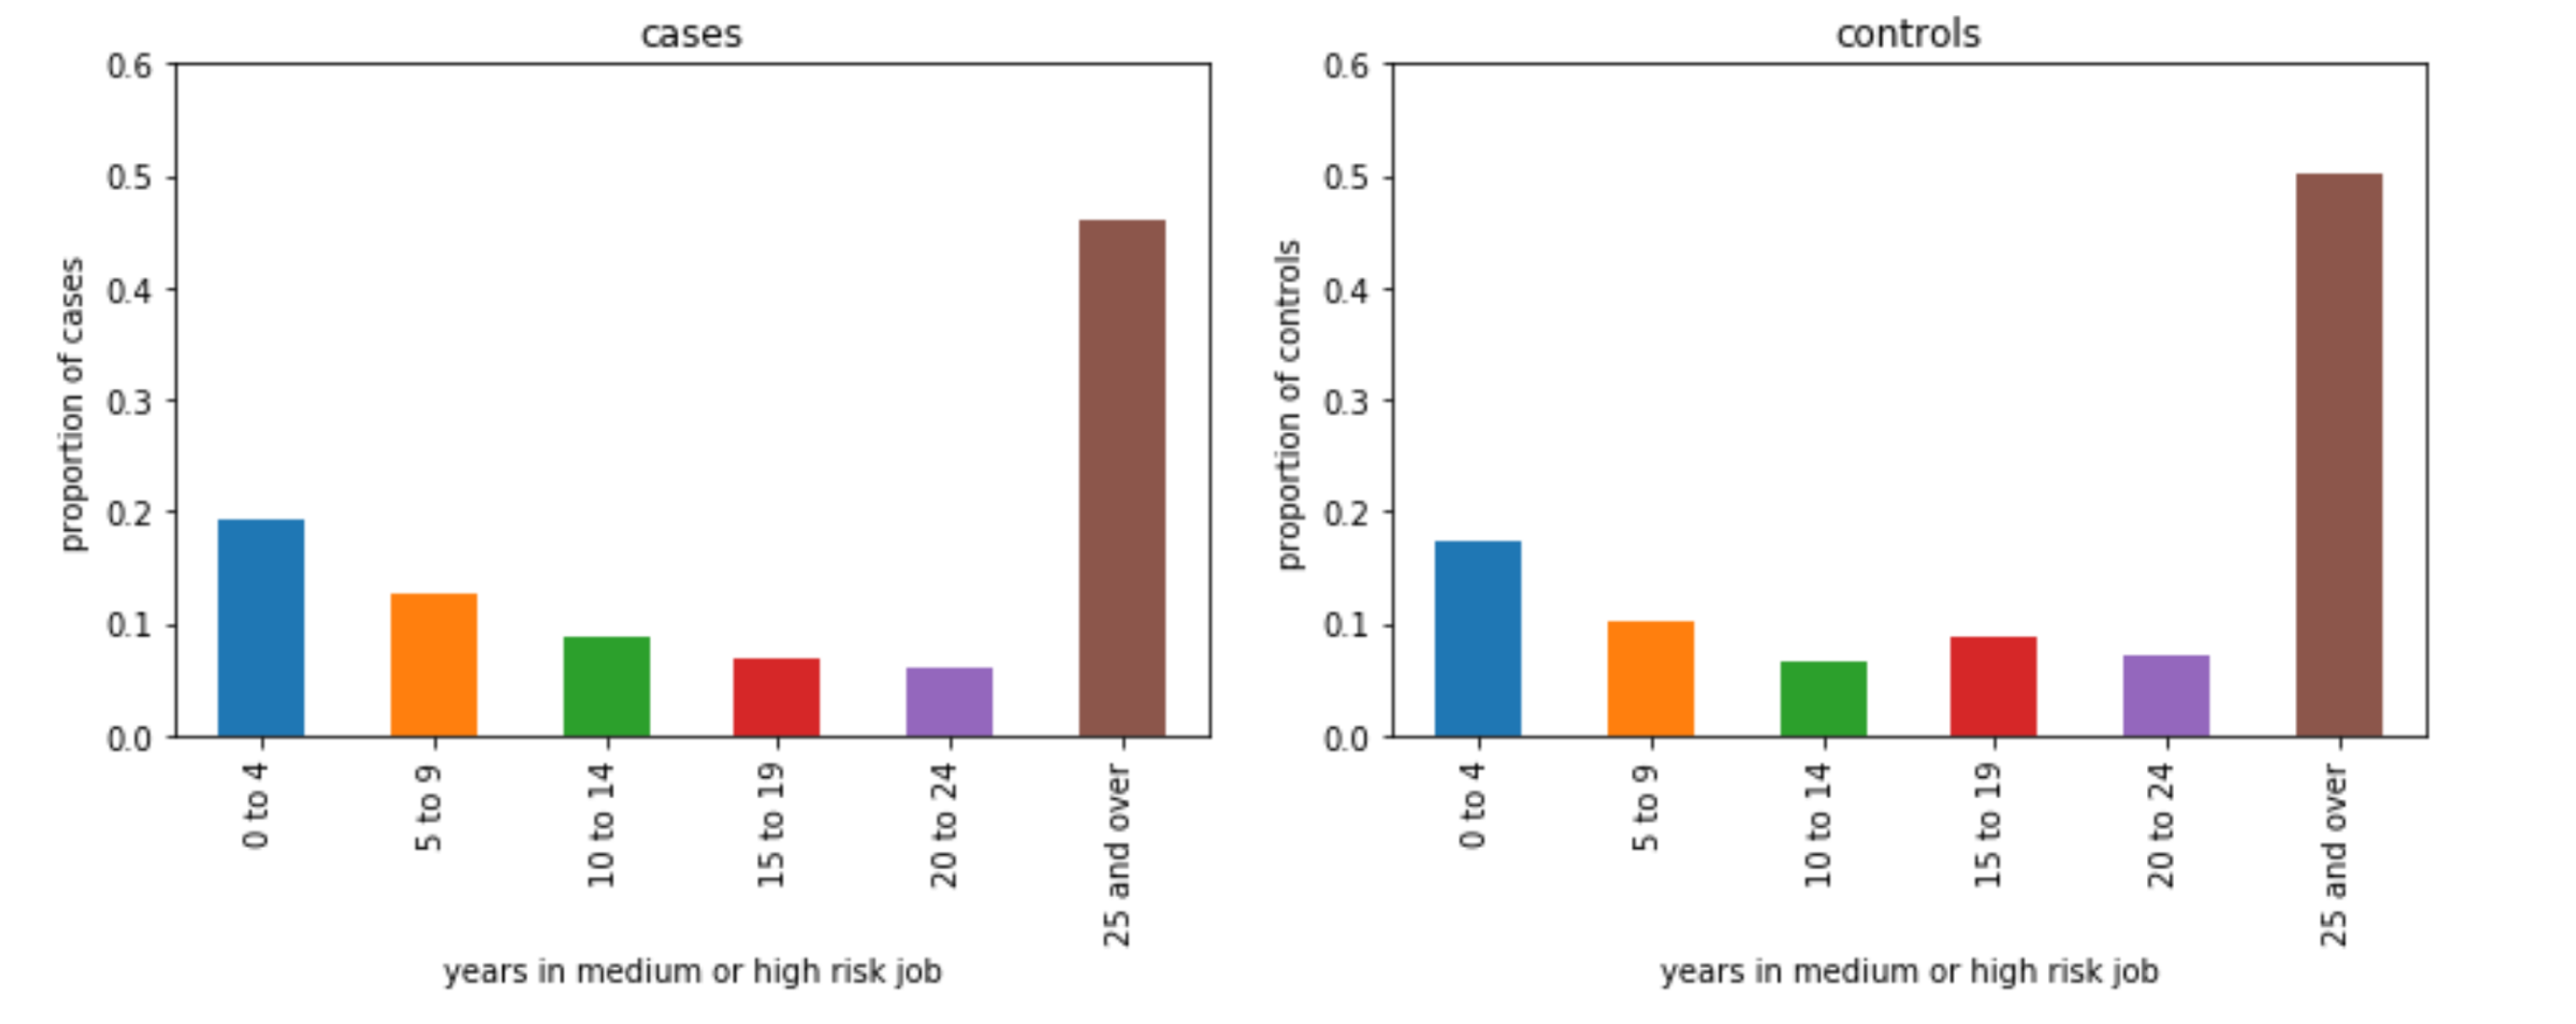
\includegraphics{source/figures/years.png}
\caption{Years in a medium or high risk asbestos exposure job for cases
and controls. Analysis limited to participants ever having had a medium
or high risk asbestos exposure job (N=492).}
\end{figure}

Cases and controls lived an average of 28km and 16km respectively from
their recruiting hospital, measured by calculating the distance between
the postcode centroid of the participants general practice and the
postcode centroid of the hospital. Living further away from the hospital
correlated with being a case, r\ensuremath{=}0.22, 95\% CI = 0.16-0.29,
p \ensuremath{<} 0.001 and weakly correlated with reduced asbestos
exposure, r=-0.06, 95\%CI = -0.13-0, p=0.05. To investigate this further
I performed a sensitivity analysis limited to participants living within
10km of their recruiting hospital (Table 6.13 and 6.14).

\hypertarget{table-6.13-sensitivity-analysis-limited-to-participants-within-10km-of-the-hospital-occupational-asbestos-exposure-inferred-by-job-title-and-ipf-risk-ever-vs-never}{%
\subsubsection{Table 6.13: Sensitivity analysis (limited to participants
within 10km of the hospital): Occupational asbestos exposure (inferred
by job title) and IPF risk (ever vs
never)}\label{table-6.13-sensitivity-analysis-limited-to-participants-within-10km-of-the-hospital-occupational-asbestos-exposure-inferred-by-job-title-and-ipf-risk-ever-vs-never}}

\begin{longtable}[]{@{}lllll@{}}
\toprule
\begin{minipage}[b]{0.06\columnwidth}\raggedright
\strut
\end{minipage} & \begin{minipage}[b]{0.10\columnwidth}\raggedright
Cases (\%)\strut
\end{minipage} & \begin{minipage}[b]{0.12\columnwidth}\raggedright
Controls (\%)\strut
\end{minipage} & \begin{minipage}[b]{0.29\columnwidth}\raggedright
Unadjusted OR (95\%CI; p-value)\strut
\end{minipage} & \begin{minipage}[b]{0.28\columnwidth}\raggedright
Adjusted OR\textsuperscript{1} (95\%CI; p-value)\strut
\end{minipage}\tabularnewline
\midrule
\endhead
\begin{minipage}[t]{0.06\columnwidth}\raggedright
ever\strut
\end{minipage} & \begin{minipage}[t]{0.10\columnwidth}\raggedright
111(73)\strut
\end{minipage} & \begin{minipage}[t]{0.12\columnwidth}\raggedright
180(64)\strut
\end{minipage} & \begin{minipage}[t]{0.29\columnwidth}\raggedright
1.46(0.95-2.26; 0.08)\strut
\end{minipage} & \begin{minipage}[t]{0.28\columnwidth}\raggedright
1.33(0.82-2.16; 0.24)\strut
\end{minipage}\tabularnewline
\begin{minipage}[t]{0.06\columnwidth}\raggedright
never\strut
\end{minipage} & \begin{minipage}[t]{0.10\columnwidth}\raggedright
42(27)\strut
\end{minipage} & \begin{minipage}[t]{0.12\columnwidth}\raggedright
100(36)\strut
\end{minipage} & \begin{minipage}[t]{0.29\columnwidth}\raggedright
1\strut
\end{minipage} & \begin{minipage}[t]{0.28\columnwidth}\raggedright
1\strut
\end{minipage}\tabularnewline
\bottomrule
\end{longtable}

\textsuperscript{1} Adjusted for age, smoking, and centre

\hypertarget{table-6.14-sensitivity-analysis-limited-to-participants-within-10km-of-the-hospital-occupational-asbestos-exposure-inferred-by-job-title-and-ipf-risk-categories-of-exposure}{%
\subsubsection{Table 6.14: Sensitivity analysis (limited to participants
within 10km of the hospital): Occupational asbestos exposure (inferred
by job title) and IPF risk (categories of
exposure)}\label{table-6.14-sensitivity-analysis-limited-to-participants-within-10km-of-the-hospital-occupational-asbestos-exposure-inferred-by-job-title-and-ipf-risk-categories-of-exposure}}

\begin{longtable}[]{@{}lllll@{}}
\toprule
\begin{minipage}[b]{0.20\columnwidth}\raggedright
Category\strut
\end{minipage} & \begin{minipage}[b]{0.08\columnwidth}\raggedright
Cases (\%)\strut
\end{minipage} & \begin{minipage}[b]{0.10\columnwidth}\raggedright
Controls (\%)\strut
\end{minipage} & \begin{minipage}[b]{0.24\columnwidth}\raggedright
Unadjusted OR (95\%CI; p-value)\strut
\end{minipage} & \begin{minipage}[b]{0.23\columnwidth}\raggedright
Adjusted OR\textsuperscript{1} (95\%CI; p-value)\strut
\end{minipage}\tabularnewline
\midrule
\endhead
\begin{minipage}[t]{0.20\columnwidth}\raggedright
high-risk non-construction\strut
\end{minipage} & \begin{minipage}[t]{0.08\columnwidth}\raggedright
23(15)\strut
\end{minipage} & \begin{minipage}[t]{0.10\columnwidth}\raggedright
35(13)\strut
\end{minipage} & \begin{minipage}[t]{0.24\columnwidth}\raggedright
1.62(0.75-3.51;0.22)\strut
\end{minipage} & \begin{minipage}[t]{0.23\columnwidth}\raggedright
1.05(0.44-2.52;0.9)\strut
\end{minipage}\tabularnewline
\begin{minipage}[t]{0.20\columnwidth}\raggedright
high-risk construction\strut
\end{minipage} & \begin{minipage}[t]{0.08\columnwidth}\raggedright
47(31)\strut
\end{minipage} & \begin{minipage}[t]{0.10\columnwidth}\raggedright
80(29)\strut
\end{minipage} & \begin{minipage}[t]{0.24\columnwidth}\raggedright
1.45(0.74-2.83;0.23)\strut
\end{minipage} & \begin{minipage}[t]{0.23\columnwidth}\raggedright
1.21(0.58-2.52;0.62)\strut
\end{minipage}\tabularnewline
\begin{minipage}[t]{0.20\columnwidth}\raggedright
medium risk industrial\strut
\end{minipage} & \begin{minipage}[t]{0.08\columnwidth}\raggedright
41(27)\strut
\end{minipage} & \begin{minipage}[t]{0.10\columnwidth}\raggedright
65(23)\strut
\end{minipage} & \begin{minipage}[t]{0.24\columnwidth}\raggedright
1.55(0.78-3.09;0.21)\strut
\end{minipage} & \begin{minipage}[t]{0.23\columnwidth}\raggedright
0.93(0.43-2.04;0.86)\strut
\end{minipage}\tabularnewline
\begin{minipage}[t]{0.20\columnwidth}\raggedright
low risk industrial\strut
\end{minipage} & \begin{minipage}[t]{0.08\columnwidth}\raggedright
25(16)\strut
\end{minipage} & \begin{minipage}[t]{0.10\columnwidth}\raggedright
58(21)\strut
\end{minipage} & \begin{minipage}[t]{0.24\columnwidth}\raggedright
1.06(0.51-2.21;0.87)\strut
\end{minipage} & \begin{minipage}[t]{0.23\columnwidth}\raggedright
0.69(0.31-1.59;0.39)\strut
\end{minipage}\tabularnewline
\begin{minipage}[t]{0.20\columnwidth}\raggedright
office\strut
\end{minipage} & \begin{minipage}[t]{0.08\columnwidth}\raggedright
17(11)\strut
\end{minipage} & \begin{minipage}[t]{0.10\columnwidth}\raggedright
42(15)\strut
\end{minipage} & \begin{minipage}[t]{0.24\columnwidth}\raggedright
1\strut
\end{minipage} & \begin{minipage}[t]{0.23\columnwidth}\raggedright
1\strut
\end{minipage}\tabularnewline
\bottomrule
\end{longtable}

\textsuperscript{1} Adjusted for age, smoking, and centre

To investigate cumulative `dose' of exposure based on job title a score
was assigned based on asbestos exposure risk category of each job as
follows:

\begin{itemize}
\tightlist
\item
  high-risk non-construction : 2
\item
  high-risk construction : 2
\item
  medium risk industrial : 1
\item
  low risk industrial : 0
\item
  office : 0
\end{itemize}

Scores were then multiplied for each job by the duration in years of the
job and then summed at participant level. See Table 6.15 and Figure 6.8.

\hypertarget{table-6.15-cumulative-dose-based-on-occupational-asbestos-exposure-inferred-by-job-title}{%
\subsubsection{Table 6.15: Cumulative `dose' based on occupational
asbestos exposure (inferred by job
title)}\label{table-6.15-cumulative-dose-based-on-occupational-asbestos-exposure-inferred-by-job-title}}

\begin{longtable}[]{@{}lllllllll@{}}
\toprule
& N & mean & std & min & 25\% & 50\% & 75\% & max\tabularnewline
\midrule
\endhead
cases & 494 & 23.9 & 30.8 & 0 & 0 & 9 & 40 & 126\tabularnewline
controls & 466 & 24 & 30.4 & 0 & 0 & 6.5 & 42 & 118\tabularnewline
\bottomrule
\end{longtable}

\begin{figure}
\centering
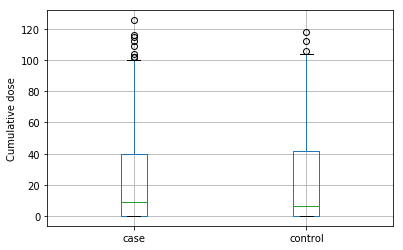
\includegraphics{source/figures/dose.png}
\caption{Boxplot of cumulative asbestos exposure estimates (inferred
from job title) for cases and controls (N=960)}
\end{figure}

Three hundred and ten (63\%) IPF cases initially presented to their
doctor with cough and 306 (62\%) with breathlessness (91 patients
presented with cough and breathlessness). Fifteen (3\%) cases and 42
(9\%) controls reported ever taking a medication suspected of causing
usual interstitial pneumonia (amiodarone, azathioprine, bleomycin,
flecainide, gefitinib, ifosfamide, melphalan, and
nitrofurantoin).{[}@Bonniaud2014{]}

Four hundred and fourteen (83\%) cases and 441 (95\%) controls reported
one or more comorbidities. The most commonly reported comorbidities
(occurring in at least 10 cases or controls) occurred at a similar
frequency in cases and controls and included hypertension, type II
diabetes mellitus, hypercholesterolemia, ischaemic heart disease, atrial
fibrillation, COPD, osteoarthritis, and prostate cancer. Rheumatoid
arthritis was reported in 18 cases, approximately 2\% of cases reporting
a comorbidity, and in 9 controls, approximately 1\% of controls
reporting a comorbidity. Gastro-oesophageal reflux disease (GORD) was
reported in 14 cases, approximately 1.5\% of cases reporting a
comorbidity, and in 2 controls, approximately 0.5\% of controls
reporting a comorbidity.

Dyspnoea, as measured by the mMRC dyspnoea scale was associated with
case-status, smoking status, genotype, and asbestos exposure. Pearson's
correlation coefficient for IPF was 0.49 (95\%CI 0.44-0.53,
p\ensuremath{<}0.001), ever smoking was 0.16 (95\%CI 0.09-0.23,
p\ensuremath{<}0.001), pack-years smoked was 0.2 (95\%CI 0.13-0.26,
p\ensuremath{<}0.001), genotype 0.2 (95\%CI 0.13-0.27,
p\ensuremath{<}0.001), ever held a medium or high risk asbestos exposure
job title 0.09 (95\%CI 0.02-0.16, p=0.02), and 0.15 (95\%CI 0.08-0.21,
p\ensuremath{<}0.001) for having a fibre-ml.year estimate \textgreater{}
25. See Table 6.16 and 6.17 for ordinal logistic regression results.

\newpage

\hypertarget{table-6.16-ordinal-logistic-regression-for-mmrc-score-and-ever-exposed-to-asbestos}{%
\subsubsection{Table 6.16: Ordinal logistic regression for mMRC score
and ever exposed to
asbestos}\label{table-6.16-ordinal-logistic-regression-for-mmrc-score-and-ever-exposed-to-asbestos}}

\begin{longtable}[]{@{}lll@{}}
\toprule
& Unadjusted OR (95\%CI; p-value) & Adjusted OR\textsuperscript{1}
(95\%CI; p-value)\tabularnewline
\midrule
\endhead
case & 6.94(5.38-9; \ensuremath{<}0.001) & 6.8 (5.25-8.8;
\ensuremath{<}0.001)\tabularnewline
pack-years & 1.01(1-1.02;\ensuremath{<}0.001) & 1.02(1.01-1.02;
\ensuremath{<}0.001)\tabularnewline
ever exposed\textsuperscript{2} & 1.48(1.17-1.87; \ensuremath{<}0.001) &
1.44(1.12-1.84; 0.004)\tabularnewline
\bottomrule
\end{longtable}

\textsuperscript{1} Adjusted for age, smoking (pack-years), and case
status \textsuperscript{2} Ever exposed to a high or medium asbestos
exposure job (inferred from job title)

\hypertarget{table-6.17-ordinal-logistic-regression-for-mmrc-score-and-for-categories-of-asbestos-exposure}{%
\subsubsection{Table 6.17: Ordinal logistic regression for mMRC score
and for categories of asbestos
exposure}\label{table-6.17-ordinal-logistic-regression-for-mmrc-score-and-for-categories-of-asbestos-exposure}}

\begin{longtable}[]{@{}lll@{}}
\toprule
Category & Unadjusted OR(95\%CI;p-value) & Adjusted
OR\textsuperscript{1}(95\%CI;p-value)\tabularnewline
\midrule
\endhead
high-risk non-construction & 2.21(1.43-3.44;\ensuremath{<}0.001) &
1.92(1.2-3.03;0.006)\tabularnewline
high-risk construction & 1.9(1.31-2.74;0.001) &
1.89(1.29-2.78;0.001)\tabularnewline
medium risk industrial & 1.36(0.94-1.98;0.103) &
1.28(0.87-1.89;0.21)\tabularnewline
low risk industrial & 1.29(0.88-1.9;0.19) &
1.24(0.82-1.87;0.29)\tabularnewline
office & 1 & 1\tabularnewline
\bottomrule
\end{longtable}

\textsuperscript{1} Adjusted for age, smoking (pack-years), and case
status

Among the 818 genotyped participants the MUC5b rs35705950 minor allele
frequency (MAF) was 35\% in cases (N=395) and 12\% in controls (N=423).
Subsets of genotyped cases with asbestos and smoking exposure had higher
MAFs then did genotyped cases who had exposure to asbestos or smoking
alone. See Table 6.18.

\newpage

\hypertarget{table-6.18-rs35705950-maf-for-genotyped-cases-case-subsets-and-controls-n}{%
\subsubsection{Table 6.18: rs35705950 MAF for genotyped cases, case
subsets, and controls
(N)}\label{table-6.18-rs35705950-maf-for-genotyped-cases-case-subsets-and-controls-n}}

rs35705950 MAF for genotyped cases, case subsets, and controls
(N)\textsuperscript{1}

\begin{longtable}[]{@{}llllllll@{}}
\toprule
\begin{minipage}[b]{0.05\columnwidth}\raggedright
\strut
\end{minipage} & \begin{minipage}[b]{0.05\columnwidth}\raggedright
IPF (395)\strut
\end{minipage} & \begin{minipage}[b]{0.09\columnwidth}\raggedright
IPF smoker (299)\strut
\end{minipage} & \begin{minipage}[b]{0.11\columnwidth}\raggedright
IPF asbestos exposed (267)\strut
\end{minipage} & \begin{minipage}[b]{0.11\columnwidth}\raggedright
IPF \textgreater25 fml-yrs (35)\strut
\end{minipage} & \begin{minipage}[b]{0.15\columnwidth}\raggedright
IPF asbestos exposed AND smoker (214)\strut
\end{minipage} & \begin{minipage}[b]{0.14\columnwidth}\raggedright
IPF \textgreater25 fml-yrs AND smoker (27)\strut
\end{minipage} & \begin{minipage}[b]{0.08\columnwidth}\raggedright
Hospital controls (423)\strut
\end{minipage}\tabularnewline
\midrule
\endhead
\begin{minipage}[t]{0.05\columnwidth}\raggedright
GG\strut
\end{minipage} & \begin{minipage}[t]{0.05\columnwidth}\raggedright
152\strut
\end{minipage} & \begin{minipage}[t]{0.09\columnwidth}\raggedright
112\strut
\end{minipage} & \begin{minipage}[t]{0.11\columnwidth}\raggedright
101\strut
\end{minipage} & \begin{minipage}[t]{0.11\columnwidth}\raggedright
11\strut
\end{minipage} & \begin{minipage}[t]{0.15\columnwidth}\raggedright
76\strut
\end{minipage} & \begin{minipage}[t]{0.14\columnwidth}\raggedright
9\strut
\end{minipage} & \begin{minipage}[t]{0.08\columnwidth}\raggedright
327\strut
\end{minipage}\tabularnewline
\begin{minipage}[t]{0.05\columnwidth}\raggedright
GT\strut
\end{minipage} & \begin{minipage}[t]{0.05\columnwidth}\raggedright
212\strut
\end{minipage} & \begin{minipage}[t]{0.09\columnwidth}\raggedright
161\strut
\end{minipage} & \begin{minipage}[t]{0.11\columnwidth}\raggedright
142\strut
\end{minipage} & \begin{minipage}[t]{0.11\columnwidth}\raggedright
20\strut
\end{minipage} & \begin{minipage}[t]{0.15\columnwidth}\raggedright
117\strut
\end{minipage} & \begin{minipage}[t]{0.14\columnwidth}\raggedright
15\strut
\end{minipage} & \begin{minipage}[t]{0.08\columnwidth}\raggedright
91\strut
\end{minipage}\tabularnewline
\begin{minipage}[t]{0.05\columnwidth}\raggedright
TT\strut
\end{minipage} & \begin{minipage}[t]{0.05\columnwidth}\raggedright
31\strut
\end{minipage} & \begin{minipage}[t]{0.09\columnwidth}\raggedright
26\strut
\end{minipage} & \begin{minipage}[t]{0.11\columnwidth}\raggedright
24\strut
\end{minipage} & \begin{minipage}[t]{0.11\columnwidth}\raggedright
4\strut
\end{minipage} & \begin{minipage}[t]{0.15\columnwidth}\raggedright
21\strut
\end{minipage} & \begin{minipage}[t]{0.14\columnwidth}\raggedright
3\strut
\end{minipage} & \begin{minipage}[t]{0.08\columnwidth}\raggedright
5\strut
\end{minipage}\tabularnewline
\begin{minipage}[t]{0.05\columnwidth}\raggedright
MAF\strut
\end{minipage} & \begin{minipage}[t]{0.05\columnwidth}\raggedright
35\strut
\end{minipage} & \begin{minipage}[t]{0.09\columnwidth}\raggedright
36\strut
\end{minipage} & \begin{minipage}[t]{0.11\columnwidth}\raggedright
36\strut
\end{minipage} & \begin{minipage}[t]{0.11\columnwidth}\raggedright
40\strut
\end{minipage} & \begin{minipage}[t]{0.15\columnwidth}\raggedright
37\strut
\end{minipage} & \begin{minipage}[t]{0.14\columnwidth}\raggedright
39\strut
\end{minipage} & \begin{minipage}[t]{0.08\columnwidth}\raggedright
12\strut
\end{minipage}\tabularnewline
\bottomrule
\end{longtable}

\textsuperscript{1} Genotype of MUC5Brs35705950, T is minor allele. MAF
is minor allele frequency (\%).

A history of ever having smoked and ever having had a high or medium
risk job for asbestos exposure was associated with increased risk of IPF
when participants also had the minor allele of MUC5b rs35705950, OR
4.6(1.5-14, p=0.01). No significant risk was observed for ever smoking
or ever being asbestos exposed alone when stratifying for genotype. See
Table 6.19, 6.20, and 6.21.

\newpage

\hypertarget{table-6.19-logistic-regression-of-ever-smoking-and-ever-exposed-to-occupational-asbestos-inferred-by-job-title-stratified-by-muc5b-rs35705950-genotype}{%
\subsubsection{Table 6.19: Logistic regression of ever smoking and ever
exposed to occupational asbestos (inferred by job title) stratified by
MUC5B rs35705950
genotype}\label{table-6.19-logistic-regression-of-ever-smoking-and-ever-exposed-to-occupational-asbestos-inferred-by-job-title-stratified-by-muc5b-rs35705950-genotype}}

\begin{longtable}[]{@{}ll@{}}
\toprule
Exposure & OR (95\% CI; p-value)\textsuperscript{1}
\textsuperscript{2}\tabularnewline
\midrule
\endhead
Ever smoker and ever asbestos exposed (all) & 1.73 (0.91-3.3,
0.09)\tabularnewline
Ever smoker and ever asbestos exposed, GT or TT\textsuperscript{3} & 4.6
(1.5-14, 0.01)\tabularnewline
Ever smoker and ever asbestos exposed, GG\textsuperscript{3} & 0.94
(0.38-2.3, 0.9)\tabularnewline
\bottomrule
\end{longtable}

\textsuperscript{1} additive model, adjusted for age and smoking
\textsuperscript{2} analysis limited to genotyped participants (N=818)
\textsuperscript{3} Genotype of MUC5B rs35705950, T is minor allele

\hypertarget{table-6.20-logistic-regression-of-ever-smoking-stratified-by-muc5b-rs35705950-genotype}{%
\subsubsection{Table 6.20: Logistic regression of ever smoking
stratified by MUC5B rs35705950
genotype}\label{table-6.20-logistic-regression-of-ever-smoking-stratified-by-muc5b-rs35705950-genotype}}

\begin{longtable}[]{@{}ll@{}}
\toprule
Exposure & OR (95\% CI; p-value)\textsuperscript{1}
\textsuperscript{2}\tabularnewline
\midrule
\endhead
Ever smoker (all) & 1.45 (1.06-1.99, 0.02)\tabularnewline
Ever smoker, GT or TT\textsuperscript{3} & 1.66 (0.97-2.84,
0.06)\tabularnewline
Ever smoker, GG\textsuperscript{3} & 1.27 (0.83-1.96,
0.28)\tabularnewline
\bottomrule
\end{longtable}

\textsuperscript{1} additive model, adjusted for age \textsuperscript{2}
analysis limited to genotyped participants (N=818) \textsuperscript{3}
Genotype of MUC5B rs35705950, T is minor allele

\newpage

\hypertarget{table-6.21-logistic-regression-of-ever-having-been-exposed-to-occupational-asbestos-inferred-by-job-title-stratified-by-muc5b-rs35705950-genotype}{%
\subsubsection{Table 6.21: Logistic regression of ever having been
exposed to occupational asbestos (inferred by job title) stratified by
MUC5B rs35705950
genotype}\label{table-6.21-logistic-regression-of-ever-having-been-exposed-to-occupational-asbestos-inferred-by-job-title-stratified-by-muc5b-rs35705950-genotype}}

\begin{longtable}[]{@{}ll@{}}
\toprule
Exposure & OR (95\% CI; p-value)\textsuperscript{1}
\textsuperscript{2}\tabularnewline
\midrule
\endhead
Ever asbestos exposed (all) & 1.17 (0.88-1.57, 0.29)\tabularnewline
Ever asbestos exposed, GT or TT\textsuperscript{3} & 1.62 (0.99-2.64,
0.06)\tabularnewline
Ever asbestos exposed, GG\textsuperscript{3} & 1.02 (0.68-1.53,
0.94)\tabularnewline
\bottomrule
\end{longtable}

\textsuperscript{1} additive model, adjusted for age and smoking
\textsuperscript{2} analysis limited to genotyped participants (N=818)
\textsuperscript{3} Genotype of MUC5B rs35705950, T is minor allele

A history of ever having smoked and ever having had a high or medium
risk job for asbestos exposure was associated with increased risk of IPF
when analysis was limited to include only cases with definite UIP, OR
2.33 (95\%CI 1.13-4.8, p=0.02), see Table 6.22. The association of ever
smoking and ever having medium of high risk job for asbestos exposure
with IPF risk was stronger when analysis was limited to include only
cases with definite UIP, OR 8.56 (95\%CI 2.39-30.69, p=0.001), see Table
6.23 and 6.24.

\newpage

\hypertarget{table-6.22-sensitivity-analysis-logistic-regression-of-ever-smoking-and-ever-exposed-to-occupational-asbestos-inferred-by-job-title-radiology-definite-uippossible-uip}{%
\subsubsection{Table 6.22: Sensitivity analysis logistic regression of
ever smoking and ever exposed to occupational asbestos (inferred by job
title) radiology (definite UIP/possible
UIP)}\label{table-6.22-sensitivity-analysis-logistic-regression-of-ever-smoking-and-ever-exposed-to-occupational-asbestos-inferred-by-job-title-radiology-definite-uippossible-uip}}

\begin{longtable}[]{@{}ll@{}}
\toprule
\begin{minipage}[b]{0.64\columnwidth}\raggedright
Exposure\strut
\end{minipage} & \begin{minipage}[b]{0.30\columnwidth}\raggedright
OR (95\% CI; p-value)\textsuperscript{1}\strut
\end{minipage}\tabularnewline
\midrule
\endhead
\begin{minipage}[t]{0.64\columnwidth}\raggedright
Ever smoker and ever asbestos exposed (all)\textsuperscript{2}\strut
\end{minipage} & \begin{minipage}[t]{0.30\columnwidth}\raggedright
1.85 (1.02-3.36, 0.04)\strut
\end{minipage}\tabularnewline
\begin{minipage}[t]{0.64\columnwidth}\raggedright
Ever smoker and ever asbestos exposed, definite
UIP\textsuperscript{2}\strut
\end{minipage} & \begin{minipage}[t]{0.30\columnwidth}\raggedright
2.33 (1.13-4.8, 0.02)\strut
\end{minipage}\tabularnewline
\begin{minipage}[t]{0.64\columnwidth}\raggedright
Ever smoker and ever asbestos exposed, possible
UIP\textsuperscript{2}\strut
\end{minipage} & \begin{minipage}[t]{0.30\columnwidth}\raggedright
1.71 (0.81-3.62, 0.16)\strut
\end{minipage}\tabularnewline
\bottomrule
\end{longtable}

\textsuperscript{1} additive model, adjusted for age and smoking
\textsuperscript{2} N=960 for all, 494 cases, 466 controls. 266 cases
had definite UIP, 216 had possible UIP, and 12 cases had `other'.

\newpage

\hypertarget{table-6.23-sensitivity-analysis-of-possible-uip-logistic-regression-of-ever-smoking-and-ever-exposed-to-occupational-asbestos-inferred-by-job-title-stratified-by-muc5b-rs35705950-genotype}{%
\subsubsection{Table 6.23: Sensitivity analysis of possible UIP logistic
regression of ever smoking and ever exposed to occupational asbestos
(inferred by job title) stratified by MUC5B rs35705950
genotype}\label{table-6.23-sensitivity-analysis-of-possible-uip-logistic-regression-of-ever-smoking-and-ever-exposed-to-occupational-asbestos-inferred-by-job-title-stratified-by-muc5b-rs35705950-genotype}}

\begin{longtable}[]{@{}ll@{}}
\toprule
Exposure & OR (95\% CI; p-value)\textsuperscript{1}
\textsuperscript{2}\tabularnewline
\midrule
\endhead
Ever smoker and ever asbestos exposed (all)\textsuperscript{2} & 1.44
(0.63-3.28, 0.38)\tabularnewline
Ever smoker and ever asbestos exposed, GT or TT\textsuperscript{3} &
2.87 (0.77-10.65, 0.12)\tabularnewline
Ever smoker and ever asbestos exposed, GG\textsuperscript{3} & 1.15
(0.35-3.68, 0.82)\tabularnewline
\bottomrule
\end{longtable}

\textsuperscript{1} additive model, adjusted for age and smoking
\textsuperscript{2} analysis limited to all genotyped controls (N=423)
and genotyped cases with possible UIP (N=117) (total N=600)
\textsuperscript{3} Genotype of MUC5B rs35705950, T is minor allele

\hypertarget{table-6.24-sensitivity-analysis-of-definite-uip-logistic-regression-of-ever-smoking-and-ever-exposed-to-occupational-asbestos-inferred-by-job-title-stratified-by-muc5b-rs35705950-genotype}{%
\subsubsection{Table 6.24: Sensitivity analysis of definite UIP logistic
regression of ever smoking and ever exposed to occupational asbestos
(inferred by job title) stratified by MUC5B rs35705950
genotype}\label{table-6.24-sensitivity-analysis-of-definite-uip-logistic-regression-of-ever-smoking-and-ever-exposed-to-occupational-asbestos-inferred-by-job-title-stratified-by-muc5b-rs35705950-genotype}}

\begin{longtable}[]{@{}ll@{}}
\toprule
Exposure & OR (95\% CI; p-value)\textsuperscript{1}
\textsuperscript{2}\tabularnewline
\midrule
\endhead
Ever smoker and ever asbestos exposed (all)\textsuperscript{2} & 2.54
(1.14-5.65, 0.02)\tabularnewline
Ever smoker and ever asbestos exposed, GT or TT\textsuperscript{3} &
8.56 (2.39-30.69, 0.001)\tabularnewline
Ever smoker and ever asbestos exposed, GG\textsuperscript{3} & 0.84
(0.24-2.89, 0.9)\tabularnewline
\bottomrule
\end{longtable}

\textsuperscript{1} additive model, adjusted for age and smoking
\textsuperscript{2} analysis limited to all genotyped controls (N=423)
and genotyped cases with definite UIP (N=208) (total N=631)
\textsuperscript{3} Genotype of MUC5B rs35705950, T is minor allele

\hypertarget{discussion}{%
\subsection{Discussion}\label{discussion}}

\hypertarget{findings-interpretation-implications-relations-to-others-work-limitations-strengths}{%
\subsubsection{Findings, interpretation, implications, relations to
others work, limitations,
strengths}\label{findings-interpretation-implications-relations-to-others-work-limitations-strengths}}

Ever being exposed to an occupation at high or medium risk for asbestos
exposure was common for both cases (67\%) and controls (63\%) and the
difference in the proportion exposed between cases and controls was not
significant (Table 6.4). A similar pattern was observed for categories
of exposure (Table 6.5). Eight percent of both cases and controls had
estimated cumulative asbestos fibre-ml.year exposures in excess of 25
fibre-ml.years, the Helsinki criteria exposure threshold at which cases
of asbestosis may occur.{[}@Wolff2015{]} The majority of these
participants had high or medium risk occupations as defined by job title
with carpenter being the single most common job title accounting for 5\%
of all estimates in excess of 25 fibre-ml.years.

In common with numerous previous studies I found MUC5b rs3570950 to be
strongly associated with disease in a risk allele dose-dependent fashion
OR 5 (95\% CI 3.7-6.8, p \ensuremath{<} 0.001) for GT, OR 13.3 (95\% CI
5.1-35, p \ensuremath{<} 0.001) for TT (see Table 6.7). I found no
evidence of interaction between asbestos exposure and MUC5b rs3570950.
However, I did find a significant association for having ever smoked, OR
1.4 (95\%CI 1-1.8, p = 0.03) and for having ever smoked and having ever
had a high or medium asbestos exposure risk based on job title, OR 1.9
(95\%CI 1.03-3.36, p = 0.04). Sensitivity analyses including limiting
jobs considered to only those that ended before 1980, considering only
jobs with a duration greater than five years, considering only
participants living within 10km of their recruiting hospital, and
considering cumulative exposure `dose' based on summing years in
different asbestos exposure risk categories (assigned by job title) at
participant level, were all non-significant. In an unplanned secondary
analysis I also found a significant association self reported
occupational exposure to stone dust and IPF, OR 2.9(1.3-6.7; 0.01).

After controlling for case and smoking status a high or medium risk job
for asbestos exposure was associated with dyspnoea, measured using
ordinal logistic regression and mMRC dyspnoea score, OR 1.44(1.12-1.84;
p=0.004). The strength of association between asbestos exposure and
dyspnoea increased with increasing categories of asbestos exposure risk.
I found evidence suggesting an interaction between asbestos exposure, as
measured by ever having a job at medium or high risk for asbestos
exposure, and ever having smoked, on IPF risk, OR 1.9 (95\%CI 1.03-3.36,
p=0.04). I found evidence supporting the risk of the interaction between
ever smoking and ever having a high or medium risk asbestos exposure
job, being mediated by MUC5b promoter variant rs3505950 genotype, OR 4.6
(95\%CI 1.5-14, p=0.01) by stratifying for genotype, see Table 6.19. In
a sensitivity analysis using a strict case definition of definite UIP
the OR for IPF for those exposed to smoking and asbestos was 2.33
(95\%CI 1.13-4.8, p=0.02). When using the strict case definition and
stratifying by genotype the OR for IPF for participants who had at least
one copy of the minor allele of the MUC5b promoter variant and were
exposed to smoking and asbestos was 8.56 (95\%CI 2.39-30.69, 0.001)

Eight percent of cases apparently meet the Helsinki criteria for a
diagnosis of asbestosis.{[}@Wolff2015{]} This criterion has been
criticised for failing to reflect the linear dose-response relationship,
and lack of threshold, observed in the published
literature.{[}@Stayner1997{]}{[}@Hein2007{]}{[}@Baur2016{]} Strictly,
IPF is a diagnosis of exclusion that should not be made until exposures
to asbestos, and other known causes of fibrosis, have been
excluded.{[}@Raghu2011{]}{[}@Baur2016{]} Taken to its logical conclusion
this line of argument may result in no diagnoses of IPF in the UK since
asbestos exposure is ubiquitous; the average asbestos lung burden in men
and women without occupational asbestos exposure was recently measured
at approximately 1 fibre/mg of lung tissue.{[}@Gilham2018{]} In IPFJES
the population attributable fraction (PAF) calculated using the
adjusted, non-significant, odds ratio (OR) for ever exposed and
proportion of cases ever exposed (pc) and the equation: PAF = pc(OR -
1)/OR{[}@Blanc2019{]} is about 5\%. Of note asbestosis is not
necessarily fatal{[}@Doll1985{]} and may not even be symptomatic since
diagnostic criteria require evidence of scarring of the lungs and
evidence of asbestos exposure but not the presence of
symptoms.{[}@Wolff2015{]} In this context a cut off below which exposure
is unlikely to cause significant morbidity or mortality seems
reasonable. Asbestosis can have a latency of upwards of 40
years{[}@Harding2010{]} and rates have not yet peaked in the
UK.{[}@HSE2019{]} From 1900 until around 1960 (see Figure 6.9), when
asbestos consumption in the United Kingdom peaked, the United Kingdom
had the third highest per capita asbestos consumption in the world with
only to the United States and later Australia having higher rates of
consumption.{[}@Allen2017{]} My results are likely to generalize well
globally where, with the exception of Brazil, Russian, India, Iran, and
China which continue to consume asbestos, consumption has been lower and
peaked later. Intriguingly, my results support the concept of asbestos
exposure being associated with dyspnoea independent of having IPF and
smoking which may represent a previous unrecognised patient group.

\begin{figure}
\centering
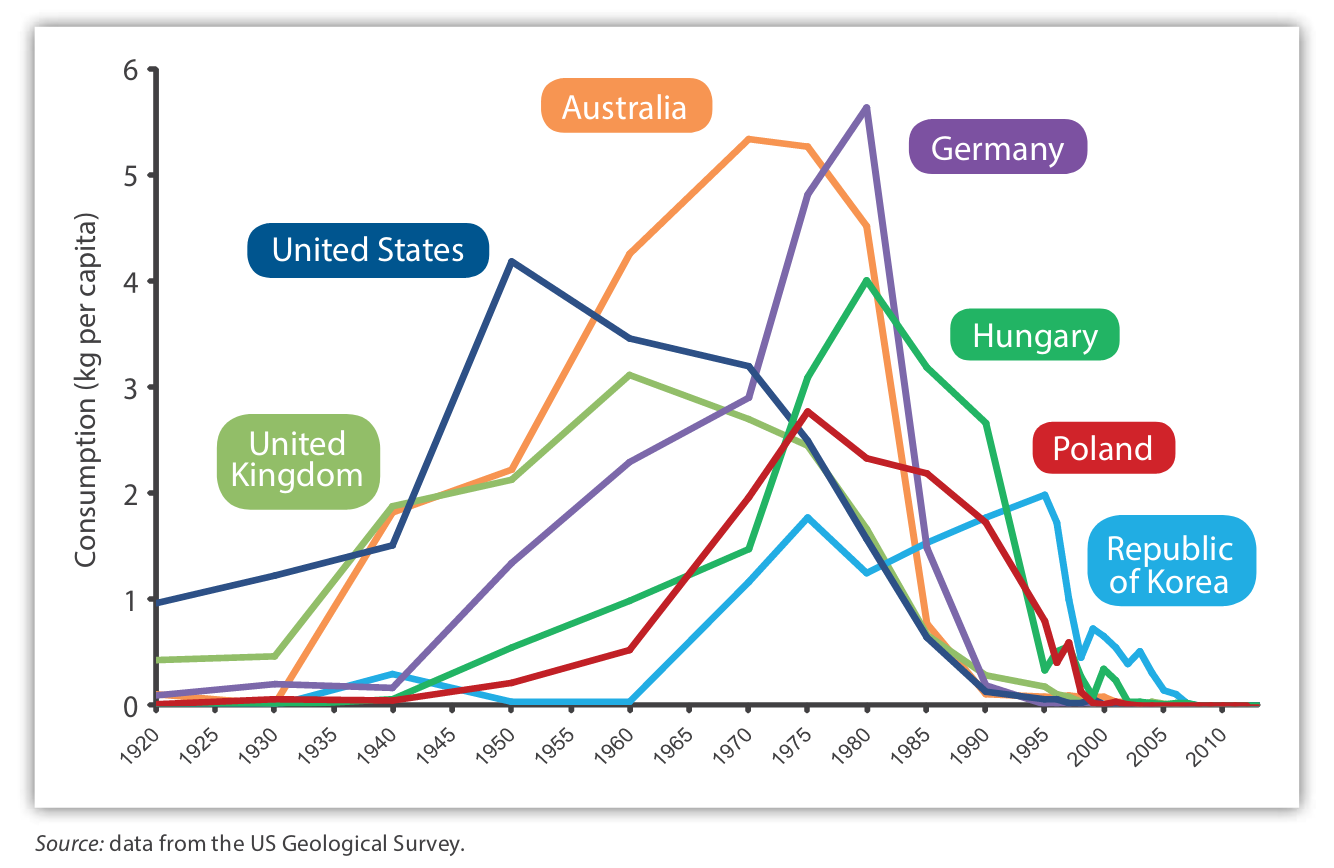
\includegraphics{source/figures/asbestos_consumption.png}
\caption{Global asbestos consumption per capita 1920-2013. (WHO 2016)}
\end{figure}

In epidemiological studies the death rate from asbestosis and prevalence
of signs and symptoms from it are both higher in cigarette smokers than
non-smokers.{[}@Doll1985{]} In mouse studies cigarette smoke and
asbestos exposure increase the production of reactive oxygen species
that are thought to be important in the pathogenesis of
asbestosis.{[}@Liu2013{]} I found evidence supporting an interaction
between ever smoking and ever having a high or medium risk asbestos
exposure job, OR 4.6 (95\%CI 1.5-14, p=0.01) when stratifying for
genotype, see Table 6.19. It is known that the minor allele of the MUC5b
promoter variant, the strongest IPF risk factor, is associated with
markedly increased MUC5b expression and that MUC5b is a dominant
constituent of the honeycomb cysts that characterise
IPF.{[}@Seibold2013{]} It is also known that asbestos exposure activates
the NLRP3 inflammasome and results in increased IL-1\ensuremath{\beta}
release (as does smoking), and that IL-1\ensuremath{\beta} release is a
potent stimulus for increased MUC5b
expression.{[}@Dostert2008{]}{[}@Mossman1998{]}{[}@Fujisawa2011{]}{[}@Kuschner1996{]}
This would add to the accumulating evidence for a MUC5b driven pulmonary
fibrosis endotype.

There is a precedent for the importance of genetic susceptibility in the
development of disease in response to asbestiform fibre inhalation;
specifically germline BAP1 mutations were discovered to be important
together with erionite exposure in the Cappadocia mesothelioma
epidemic.{[}@Testa2011{]}{[}@Emri2017{]} It is possible that there are
unmeasured genetic modifiers of asbestos exposure risk the presence, or
absence, of which is necessary for the development of disease.

Seven previous IPF case-control studies that reported on occupational
asbestos exposure found no significant
association.{[}@Scott1990{]}{[}@Hubbard1996{]}{[}@Mullen1998{]}{[}@Baumgartner2000{]}{[}@Miyake2005{]}{[}@Gustafson2007{]}{[}@Koo2017{]}
Five of these studies used population
controls{[}@Scott1990{]}{[}@Hubbard1996{]}{[}@Mullen1998{]}{[}@Baumgartner2000{]}{[}@Gustafson2007{]}
Where participation rates were reported for community controls they were
generally low, for example one study which mailed a questionnaire to
potential participants had a response rate of 32.4\% for
controls.{[}@Mullen1998{]} In another study using a mailed questionnaire
60\% of controls returned a completed questionnaire.{[}@Scott1990{]}
Controls for one of the studies were recruited from orthopaedics
practice list.{[}@Mullen1998{]} This may be undesirable as the sole
source of controls in a study of occupational exposures since, for
example, dust exposed manual workers might be over-represented because
they have more orthopaedic problems, or under-represented because they
lack healthcare access, introducing bias. Two studies recruited
respiratory inpatients.{[}@Miyake2005{]}{[}@Koo2017{]} One study did not
match cases and controls on age or sex{[}@Miyake2005{]}, and another
matched on age but not sex.{[}@Gustafson2007{]} Four
studies{[}@Scott1990{]}{[}@Mullen1998{]}{[}@Miyake2005{]}{[}@Gustafson2007{]}
relied solely on questionnaires for exposure assessment; these asked
directly about exposures, for example ``In your work, have you ever been
exposed to y?''{[}@Gustafson2007{]} Only two studies reported blinding
of assessors.{[}@Baumgartner2000{]}{[}@Koo2017{]} None of the studies
were pre-registered. None of these studies attempted to quantify
asbestos exposure or looked at gene-environment or
environment-environment interactions. Collectively these studies were at
high risk for bias arising from selection, lack of blinding, exposure
misclassification, incomplete exposure data, and selective reporting of
exposures. These studies were included in a recent meta-analysis
reporting on occupational exposures in IPF that found significant
associations occupational metal, wood, and stone dust
exposures.{[}@Blanc2019{]} The possibility of asbestos co-exposure
confounding the observed association with metal and wood dust is
intriguing; carpenters and metalplate workers, who have significant wood
and metal dust exposure are known to be high risk groups for pleural
mesothelioma, a disease almost entirely attributable to occupational
asbestos exposure.{[}@McElvenny2005{]}{[}@Rake2009{]}

There is accumulating evidence for a MUC5B driven endotype of pulmonary
fibrosis in ILD. The common MUC5b promoter variant rs35705950 is the
strongest identified genetic risk factor for IPF; minor allele frequency
\textgreater{} 0.1 in Caucasian populations, OR 4.84 (95\%CI 4.37-5.36,
p=1.18\ensuremath{\times}10\textsuperscript{-203}) in a recent genome
wide association study (GWAS) meta-analysis (total 2,668 IPF cases and
8,591 controls).{[}@Allen2019{]} Its main effect is to increase airway
expression of a distal airway glycopeptide called MUC5b
(\textgreater30-fold).{[}@Evans2016{]} MUC5b is a dominant constituent
of the honeycomb cysts that characterise IPF{[}@Seibold2013{]} and it
has recently emerged that rs3505950 is also a risk factor for
asbestosis{[}@Platenburg2020{]}, chronic hypersensitivity pneumonitis,
and rheumatoid arthritis associated ILD.{[}@Namba2019{]} As outlined
above asbestos (and silica) exposure results in production of
IL-1\ensuremath{\beta} via the NLRP3 inflammasome; smoking also
increases airway IL-1\ensuremath{\beta} levels, and
IL-1\ensuremath{\beta} is known to be a key proinflammatory cytokine in
IPF and a potent stimulus for MUC5b
expression.{[}@Kuschner1996{]}{[}@Dostert2008{]}{[}@Adair-Kirk2008{]}
Genetic variants in the NLRP3 inflammasome (e.g rs35829419) have been
found to be associated asbestosis{[}@Kukkonen2014{]} and coal workers
pneumoconiosis{[}@Ji2012{]}, and are likely to be important mediators of
IPF risk due to inhaled particles. Of note, the lungs can also be an
initiating site of rheumatoid arthritis.{[}@Catrina2016{]} Occupational
exposure to respirable crystalline silica is associated with an
increased risk of rheumatoid arthritis in men{[}@Stolt2010{]}, and
rheumatoid arthritis associated ILD (which causes UIP) is more common in
men despite rheumatoid arthritis being more common in
women.{[}@Rosenman2012{]} Genetic variants in the NLRP3 inflammasome
(e.g rs35829419) have been found to be associated with increased risks
of rheumatoid arthritis.{[}@Mathews2014{]}

A limitation of my study is that I lack comprehensive data on
participation rates. Recruiting centres were provided with screening
logs and asked to report monthly the number of eligible participants
identified, approached, and recruited. For the centres that did provide
monthly data (N=3) participation rates were high; fewer than 5\% of
participants approached declined to enroll in the study with no
significant difference between cases and controls. After enrollment 22
of 516 cases(4\%), and 45 of 511 controls(9\%) were withdrawn because
they no longer wished to take part in the study, did not respond after
we called them on three occasions, or died before the interview took
place. This gives an overall participation rate of approximately 91\%
for cases and 86\% for controls. However, recruitment was poor at
several centres; this is likely to mean that many eligible participants
were not invited to participate due to, for example, research staff
shortages.

My study has several strengths in comparison to previous case-control
studies that have investigated occupational asbestos exposure in IPF. I
assessed occupational asbestos exposure in 466 male participants, the
largest previous study assessed 149 male
participants{[}@Baumgartner2000{]}, and I surpassed the recruitment
target required for adequate power. Risk of selection bias was minimised
through the use of hospital controls and randomly sampling outpatient
clinics. Assessors were blinded to case-status during the asbestos
exposure assessment process and study design and pre-specified analyses
were registered on clincialtrial.gov (NCT03211507). Participants were
genotyped for MUC5b promoter variant rs3505950 and two validated means
of assessing asbestos exposure were used to permit quantitative and
semi-quantitative analysis, and allow assessment for gene-environment
and environment-environment interaction.

There is now a need to make use of modern techniques such as Mendelian
randomisation (MR) within a population of IPF patients with well
characterised occupational exposures. MR is a technique that uses
randomly distributed genetic variants as natural experiments to provide
evidence about putative causal relations between modifiable risk factors
and disease.{[}@Davies2018{]} Through its use of genetic variance it can
overcome problems of confounding and reverse causality. MR can be used
within a case-control study design to help triangulate suspected causal
associations.{[}@Lawlor2016{]} It could be usefully applied to IPFJES,
or similar case-control study data, to investigate interactions between
occupational silica and asbestos exposure, smoking, and NLRP3
inflammasome variants, with respect to IPF risk, in order to better
understand the aetiology of IPF and potentially identify new therapeutic
targets. See Figures 6.10{[}@Adair-Kirk2008{]} and 6.11.

\begin{figure}
\centering
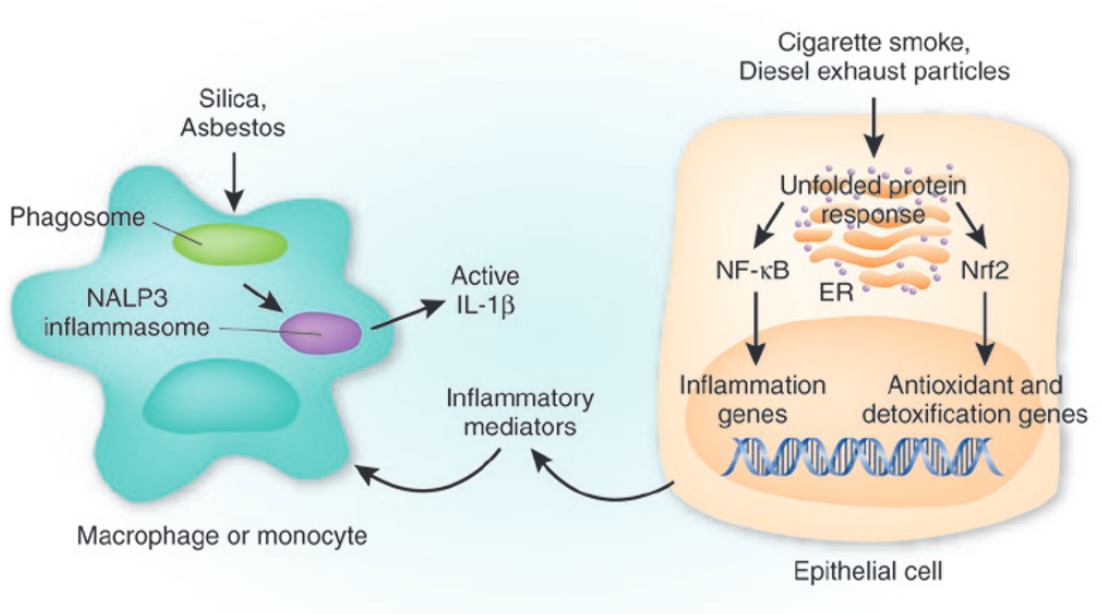
\includegraphics{source/figures/asbestos_silica_smoking.png}
\caption{Proposed pathway for particulate-induced lung inflammation and
IL-1\ensuremath{\beta} production. (Adair-Kirk 2008)}
\end{figure}

\begin{figure}
\centering
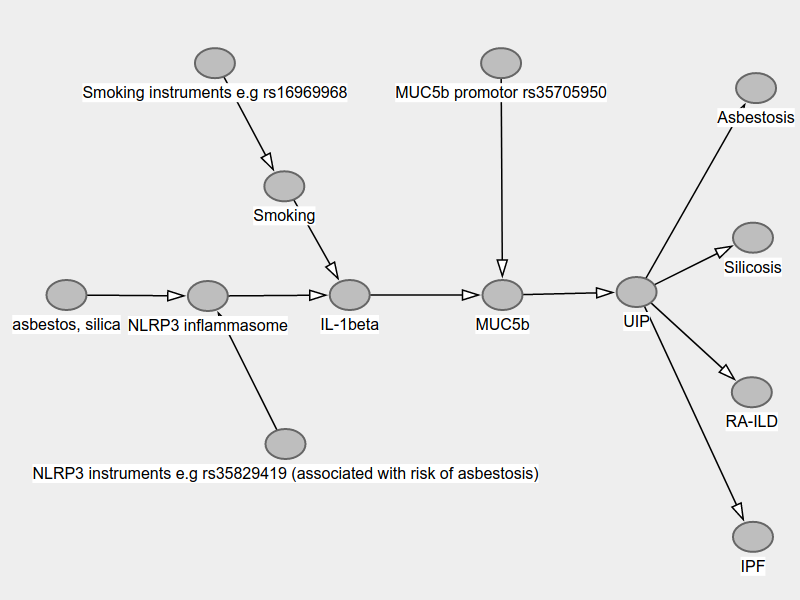
\includegraphics{source/figures/possible_pathways_mr.png}
\caption{Proposed pathway for particulate-induced NLRP3,
IL-1\ensuremath{\beta} mediated MUC5b driven pulmonary fibrosis
endotype.}
\end{figure}

\hypertarget{conclusion}{%
\subsection{Conclusion}\label{conclusion}}

The majority of men in their 70s in the UK who attend hospital have held
a high or medium risk for asbestos exposure job during their working
lifetime; estimated asbestos exposure based on validated means inferred
by job title or historic asbestos exposure reconstruction methods does
not significantly affect risk of IPF. Nonetheless, about 8\% of IPF
cases have a history of heavy occupational asbestos exposure
(\textgreater25 fibre-ml.years) that would support a diagnosis of
asbestosis based on the Helsinki criteria. Asbestos exposure alone does
not appear to be an important cause of IPF. However, asbestos exposure
does appear to interact with smoking and the minor allele of the MUC5b
promoter variant rs35705950 to increase IPF risk and this effect is
larger when analysis is limited to cases with definite UIP. Asbestos
exposure also appears to be associated with MRC dyspnoea in my study and
this association is independent of case and smoking status.
